\documentclass[MS]{iitmdiss}
\usepackage{times}
 \usepackage{t1enc}

\usepackage{graphicx}
\usepackage{epstopdf}
\usepackage[driverfallback=dvipdfm]{hyperref} % hyperlinks for references.
\usepackage{amsmath} % easier math formulae, align, subequations \ldots
%%%%%%%%%%%%%%%%
\usepackage{macros}
%%\usepackage{authblk}
\RequirePackage{algorithm}
\RequirePackage{algorithmic}
\usepackage{caption}
%\usepackage[numbers]{natbib}
%%%%%%%%%%%%%
\usepackage{enumitem}
%\usepackage{svg}

%%%%%%%%%%%%%%%%%%%%%%%%%%%%%%%%%%%%%
%\documentclass[runningheads]{llncs}
\usepackage{booktabs}   %% For formal tables:
%% http://ctan.org/pkg/booktabs
%\usepackage{subcaption} %% For complex figures with subfigures/subcaptions
%% http://ctan.org/pkg/subcaption
\usepackage{graphicx}
\usepackage{wrapfig}
\usepackage{url}
\usepackage{enumitem}
\usepackage{hyperref}
\usepackage{listings}
\usepackage{xcolor}
\usepackage{xspace}
\usepackage{inconsolata}

\usepackage{multirow}
\usepackage{amsmath}
\usepackage{cleveref}
\newcommand{\clearemptydoublepage}{\newpage{\cleardoublepage}}

\definecolor{Bittersweet}{rgb}{1.0, 0.44, 0.37}
\definecolor{MidnightBlue}{rgb}{0.0, 0.2, 0.4}
\definecolor{BrightBlue}{rgb}{0.0, 0.2, 0.7}
\definecolor{byzantine}{rgb}{0.74, 0.2, 0.64}
\definecolor{caribbeangreen}{rgb}{0.0, 0.8, 0.6}

\lstset{
	language=caml,
	basicstyle=\ttfamily\small,
	flexiblecolumns=false,
	tabsize=2,
	escapechar=',
	%basewidth={0.5em,0.45em},
	%aboveskip={3pt},
	%belowskip={3pt},
	keywordstyle=\color{Bittersweet}\bfseries,
	commentstyle=\color{blue}\itshape,
	stringstyle=\color{MidnightBlue},
	keywords=[2]{def, barrier, atomic},
	keywordstyle=[2]\color{Bittersweet}\bfseries,
	keywords=[3]{close, connect, publish, refresh, write, read},
	keywordstyle=[3]\color{byzantine}\bfseries,
	keywords=[4]{MARK, MARK_FINAL, SWEEP_EPHE},
	keywordstyle=[4]\color{caribbeangreen}\bfseries,
	classoffset=1,
	upquote=true,
	keywordstyle=\color{byzantine}\bfseries,
	classoffset=0,
	mathescape=true,
	numberstyle=\tiny\color{gray},
	numbersep=5pt
}

\lstMakeShortInline[columns=fullflexible]|

\newcommand{\ml}[1]{\lstinline[language=caml]{#1}}

\newcommand{\name}{Banyan\xspace}

%\renewcommand\UrlFont{\color{blue}\rmfamily}



\begin{document}

%%%%%%%%%%%%%%%%%%%%%%%%%%%%%%%%%%%%%%%%%%%%%%%%%%%%%%%%%%%%%%%%%%%%%%
% Title page

\title{Banyan: Coordination-free Distributed Transactions over Mergeable Types}

\author{Shashank Shekhar Dubey}

\date{July 2020}
\department{COMPUTER SCIENCE AND ENGINEERING}

%\nocite{*}
\maketitle

%%%%%%%%%%%%%%%%%%%%%%%%%%%%%%%%%%%%%%%%%%%%%%%%%%%%%%%%%%%%%%%%%%%%%%
% Certificate

%\pagebreak
%\newpage
% \ 
%\thispagestyle{empty}
%\clearpage

\clearemptydoublepage
\certificate

\vspace*{0.5in}

\noindent This is to certify that the thesis titled {\bf Banyan: Coordination-free Distributed Transactions over Mergeable Types}, submitted by {\bf Shashank Shekhar Dubey}, to the Indian Institute of Technology Madras, for the award of the degree of {\bf Master of Science (Research)}, is a bonafide
record of the research work done by him under my supervision. The contents of this thesis, in full or in parts, have not been submitted to any other Institute or University for the award of any degree or diploma.

\vspace*{1.5in}

\begin{singlespacing}
	%\hspace*{-0.25in}
	%\hspace*{1.0in} 
	%\parbox{2.0in}{
	\noindent {\bf Dr. KC Sivaramakrishnan} \\
	\noindent Research Guide \\ 
	\noindent Assistant Professor \\
	\noindent Dept. of Computer Science and Engineering\\
	\noindent IIT-Madras, Chennai - 600 036 \\
	%}  
\end{singlespacing}
\\
\\
\noindent Place: Chennai\\
Date: 


%%%%%%%%%%%%%%%%%%%%%%%%%%%%%%%%%%%%%%%%%%%%%%%%%%%%%%%%%%%%%%%%%%%%%%
% Acknowledgements
\clearemptydoublepage
\acknowledgements
%To be written.
acknowledgements here


%%%%%%%%%%%%%%%%%%%%%%%%%%%%%%%%%%%%%%%%%%%%%%%%%%%%%%%%%%%%%%%%%%%%%%
% Abstract

\abstract

\noindent KEYWORDS: \hspace*{0.5em} \parbox[t]{4.4in}{Distributed applications, Consistency, Git, Irmin, 3-way merge, Programming model}

\vspace*{24pt}

\noindent 
Programming loosely connected distributed applications is a challenging
endeavour. Loosely connected distributed applications such as geo-distributed
stores and intermittently reachable IoT devices cannot afford to coordinate
among all of the replicas in order to ensure data consistency due to
prohibitive latency costs and the impossibility of coordination if
availability is to be ensured. Thus, the state of the replicas evolves
independently, making it difficult to develop correct applications. Existing
solutions to this problem limit the data types that can be used in these
applications, which neither offer the ability to compose them to construct
more complex data types nor offer transactions.

In this paper, we describe Banyan, a distributed programming model for
developing loosely connected distributed applications. Data types in Banyan
are equipped with a three-way merge function a la Git to handle conflicts.
Banyan provides isolated transactions for grouping together individual
operations which do not require coordination among different replicas. We
instantiate Banyan over Cassandra, an off-the-shelf industrial-strength
distributed store. Several benchmarks, including a distributed build-cache,
illustrates the effectiveness of the approach.

\pagebreak

%%%%%%%%%%%%%%%%%%%%%%%%%%%%%%%%%%%%%%%%%%%%%%%%%%%%%%%%%%%%%%%%%

% Table of contents etc.
%\clearemptydoublepage
\begin{singlespace}
	\tableofcontents
	%\thispagestyle{empty}
	
	\clearemptydoublepage
	\listoftables
	\addcontentsline{toc}{chapter}{LIST OF TABLES}
	
	
	%\clearemptydoublepage
	\listoffigures
	\addcontentsline{toc}{chapter}{LIST OF FIGURES}
\end{singlespace}


%%%%%%%%%%%%%%%%%%%%%%%%%%%%%%%%%%%%%%%%%%%%%%%%%%%%%%%%%%%%%%%%%%%%%%
% Abbreviations
%\clearemptydoublepage
\abbreviations

\noindent 
\begin{tabbing}

	
	
\end{tabbing}

\pagebreak

%%%%%%%%%%%%%%%%%%%%%%%%%%%%%%%%%%%%%%%%%%%%%%%%%%%%%%%%%%%%%%%%%%%%%%
% Notations

\clearemptydoublepage
\chapter*{\centerline{NOTATIONS}}
\addcontentsline{toc}{chapter}{NOTATIONS}



\pagebreak
\clearpage

% The main text will follow from this point so set the page numbering
% to arabic from here on.

%%%%%%%%%%%%%%%%%%%%%%%%%%%%%%%%%%%%%%%%%%%%%%%%%%
%Introduction.
\clearemptydoublepage
\pagenumbering{arabic}

\chapter{Introduction}
\label{chap:introduction}
\input{Introduction.tex}
%%%%%%%%%%%%%%%%%%%%%%%%%%%%%%%%%%%%%%%%%%%%%%%%%%

%
%%%%%%%%%%%%%%%%%%%%%%%%%%%%%%%%%%%%%%%%%%%%%%%%%%%%%%%%%%%%%%%%%%%%%%
% Title page

\title{Estimation of Spectral Risk Measures}
\author{AJAY KUMAR PANDEY}

\date{JUNE 2020}
\department{COMPUTER SCIENCE AND ENGINEERING}

%\nocite{*}
\maketitle
\label{key}
%%%%%%%%%%%%%%%%%%%%%%%%%%%%%%%%%%%%%%%%%%%%%%%%%%%%%%%%%%%%%%%%%%%%%%
% Certificate
\certificate

\vspace*{0.5in}

\noindent This is to certify that the thesis titled {\bf Estimation of Spectral Risk Measures}, submitted by {\bf Ajay Kumar Pandey}, 
  to the Indian Institute of Technology, Madras, for
the award of the degree of {\bf Master of Science (by Research)}, is a bonafide
record of the research work done by him under our supervision.  The
contents of this thesis, in full or in parts, have not been submitted
to any other Institute or University for the award of any degree or
diploma.

\vspace*{1.5in}

\begin{singlespacing}
\hspace*{-0.25in}
\parbox{5in}{
\noindent {\bf Dr. Prashanth L.A.} \\
\noindent Research Advisor \\ 
\noindent Assistant Professor \\
\noindent Department of Computer Science and Engineering\\
\noindent Indian Institute of Technology Madras, 600036 \\
} 

\end{singlespacing}
\vspace*{0.25in}

\noindent Place: Chennai\\
Date: 


%%%%%%%%%%%%%%%%%%%%%%%%%%%%%%%%%%%%%%%%%%%%%%%%%%%%%%%%%%%%%%%%%%%%%%
% Acknowledgements
\acknowledgements

First and foremost, I would like to express my sincere thankfulness to my research advisor, Dr. Prashanth L.A., who has the substance of an expert: he convincingly guided and encouraged me to be professional and do the right thing even when the road got tough. The door to my advisor's office was always open whenever I ran into a trouble spot or had a question about my research or writing. Without his steady assistance, the objective of this thesis would not have been completed.

Second, I would like to thank Dr. Sanjay P. Bhat, Tata Consultancy Services Limited, Hyderabad, whose valuable feedback and ideas improved the quality of this thesis considerably. I would also like to thank my General Test Committee members, Dr. Sutanu Chakraborti, Dr. Puduru Viswanadha Reddy, and Dr. Madhu Mutyam, for their immense guidance and valuable feedback.

Third, I am also grateful to the Computer Science and Engineering department in particular and the Indian Institute of Technology Madras in general for providing an excellent environment for doing research. Furthermore, I want to thank my friends: Nirav, Sidharth, Rajendra, Pawandeep, and many others, who made my stay pleasant as ever on the campus for the last three years.

Finally, I must express my very profound gratitude to my family: my parents, my brother, and my sister, for providing me with unfailing support and continuous encouragement throughout my years of study and through the process of research and writing this thesis. This accomplishment would not have been possible without them. Thank you.

%%%%%%%%%%%%%%%%%%%%%%%%%%%%%%%%%%%%%%%%%%%%%%%%%%%%%%%%%%%%%%%%%%%%%%
% Abstract

\abstract

\noindent KEYWORDS: \hspace*{0.5em} \parbox[t]{4.4in}{Spectral risk measures, Value-at-Risk, Conditional Value-at-Risk, Estimation technique, Concentration bounds, Bounded distributions, Gaussian distribution, Exponential distribution.}

\vspace*{24pt}

\noindent 
Programming loosely connected distributed applications is a challenging
endeavour. Loosely connected distributed applications such as geo-distributed
stores and intermittently reachable IoT devices cannot afford to coordinate
among all of the replicas in order to ensure data consistency due to
prohibitive latency costs and the impossibility of coordination if
availability is to be ensured. Thus, the state of the replicas evolves
independently, making it difficult to develop correct applications. Existing
solutions to this problem limit the data types that can be used in these
applications, which neither offer the ability to compose them to construct
more complex data types nor offer transactions.

In this paper, we describe Banyan, a distributed programming model for
developing loosely connected distributed applications. Data types in Banyan
are equipped with a three-way merge function a la Git to handle conflicts.
Banyan provides isolated transactions for grouping together individual
operations which do not require coordination among different replicas. We
instantiate Banyan over Cassandra, an off-the-shelf industrial-strength
distributed store. Several benchmarks, including a distributed build-cache,
illustrates the effectiveness of the approach.

\pagebreak

%%%%%%%%%%%%%%%%%%%%%%%%%%%%%%%%%%%%%%%%%%%%%%%%%%%%%%%%%%%%%%%%%
% Table of contents etc.

\begin{singlespace}
\tableofcontents
\thispagestyle{empty}

\listoftables
\addcontentsline{toc}{chapter}{LIST OF TABLES}
\listoffigures
\addcontentsline{toc}{chapter}{LIST OF FIGURES}
\end{singlespace}


%%%%%%%%%%%%%%%%%%%%%%%%%%%%%%%%%%%%%%%%%%%%%%%%%%%%%%%%%%%%%%%%%%%%%%
% Abbreviations
\abbreviations

\noindent 
\begin{tabbing}
xxxxxxxxxxx \= xxxxxxxxxxxxxxxxxxxxxxxxxxxxxxxxxxxxxxxxxxxxxxxx \kill
%\textbf{IITM}   \> Indian Institute of Technology, Madras \\
%\textbf{MS}   \> Master of Science (by Research) \\
%\textbf{RL} \> Reinforcement Learning \\
\textbf{OR} \> Operation Research\\
\textbf{AI} \> Artificial Intelligence  \\
\textbf{VaR} \> Value-at-Risk \\
\textbf{CVaR} \> Conditional Value-at-Risk \\
\textbf{CPT} \> Cummulative Prospect Theory  \\
\textbf{SRM} \> Spectral Risk Measures \\
\textbf{EDF} \> Empirical Distribution Function \\
\textbf{SR} \> Successive Rejects \\
\textbf{SUMO} \> Simulation of Urban Mobility \\
%\textbf{i.i.d.} \> Independent and identically distributed \\
%\textbf{r.v.} \> Random variable \\
\textbf{MVRM} \> Mean-Variance Risk Measure \\
\textbf{PDF} \> Probability density function \\
\textbf{CDF} \> Cumulative distribution function \\
\textbf{} \>  \\
\textbf{} \>  \\
\textbf{} \>  \\

\end{tabbing}

\pagebreak

%%%%%%%%%%%%%%%%%%%%%%%%%%%%%%%%%%%%%%%%%%%%%%%%%%%%%%%%%%%%%%%%%%%%%%
%% Notation
%
%\chapter*{\centerline{NOTATION}}
%\addcontentsline{toc}{chapter}{NOTATION}
%
%\begin{singlespace}
%\begin{tabbing}
%xxxxxxxxxxx \= xxxxxxxxxxxxxxxxxxxxxxxxxxxxxxxxxxxxxxxxxxxxxxxx \kill
%\textbf{$\varphi(\cdot)$} \> risk aversion function\\
%\textbf{$\mu$}  \> mean\\
%\textbf{${\sigma}^2$}  \> variance \\
%%\textbf{$\beta$}   \> Confidence level \\
%%\textbf{$\alpha$}   \> Confidence level \\
%\textbf{$\mathrm{V_\beta(X)}$} \> $\mathrm{VaR}$ at the level $\beta$ of r.v. $X$, see definition \ref{def:var}.\\
%\textbf{$\mathrm{C_\beta(X)}$} \> $\mathrm{CVaR}$ at the level $\beta$ of r.v. $X$, see definition \ref{def:cvar} \\
%\textbf{$\mathrm{S(X)}$} \> $\mathrm{SRM}$ of r.v. $X$, see definition \ref{def:srm}. \\
%\textbf{$\widehat{\mathrm{V}}_{n, \beta}$} \> Estimation of $\mathrm{VaR}$ at the level $\beta$\\
%\textbf{$\mathrm{\widehat{C}_{\alpha,m}}$} \> Estimation of $\mathrm{VaR}$ at the level $\beta$\\
%\end{tabbing}
%\end{singlespace}
%
%\pagebreak
%\clearpage

% The main text will follow from this point so set the page numbering
% to arabic from here on.
\pagenumbering{arabic}
%%%%%%%%%%%
%%%%%%%%%%%%%
%%%%%%%%%%%

%%%%%%%%%%%%%%%%%%%%%%%%%%%%%%%%%%%%%%%%%%%%%%%%%%
%Introduction.
%\clearemptydoublepage
%\pagenumbering{arabic}

%\chapter{Introduction}
%\label{chap:introduction}
%\input{Introduction.tex}
%%%%%%%%%%%%%%%%%%%%%%%%%%%%%%%%%%%%%%%%%%%%%%%%%%
%\input{Introduction.tex}

%%%%%%%%%%%%%%%%%%%%%%%%%%%%%%%%%%%%%%%%%%%%%%%%%%
%Motivation.
\clearemptydoublepage
%\pagenumbering{arabic}

\chapter{Motivation}
\label{chap:motivation}
\section{A Distributed Build Cache}
\label{sec:motivation}

A distributed build cache enables a team of developers and/or a continuous
integration (CI) system to reuse the build artefacts between several builds.
Such a facility is provided by modern build tools such as Gradle~\cite{Gradle}
and Bazel~\cite{Bazel}, which can store and retrieve build artefacts from cloud
storage services such as Amazon S3 or Google Cloud Storage. Consider the
challenge of building a distributed build cache for OCaml packages. Let us
assume that the builds are reproducible -- that is, independent builds of the same source
files yield the same artefact. In addition to storing the artefacts, it would
be useful to gather statistics about the artefacts such as creation time, last
accessed time and number of cache hits. Such information may be used in the
cache eviction policy or replicating artefacts across several sites for
increased availability. While an artefact itself is reproducible, care must be
taken to ensure that the statistics are consistent. For the sake of exposition,
we will assume that all the build hosts use the same operating system and
compiler version.

\subsection{Mergeable types}

Let us build this distributed cache using \name, implementing in OCaml. At its
heart, \name is a distributed key-value store. The keys in \name are
\emph{paths}, represented as list of strings. The values are algebraic data
types equipped a merge function that reconciles conflicting updates. In this
example, we will use the following schema:
\lstinline[breaklines=true]{[<pkg_name>; <version>; <kind>; <filename>]} for
the keys, where |<kind>| is either |lib| indicating binary artefact or
|stats| indicating statistics about the artefact. The value type is given
below:
\begin{lstlisting}[language=caml]
type timestamp = float
type value =
	| B of bigarray  (*binary artefact*)
	| S of timestamp (*created*) * timestamp (*last accessed*)
	     * int (*hits*)
\end{lstlisting}

\begin{wrapfigure}{r}{0.45\textwidth}
	\vspace{-0.8cm}
	\centering
	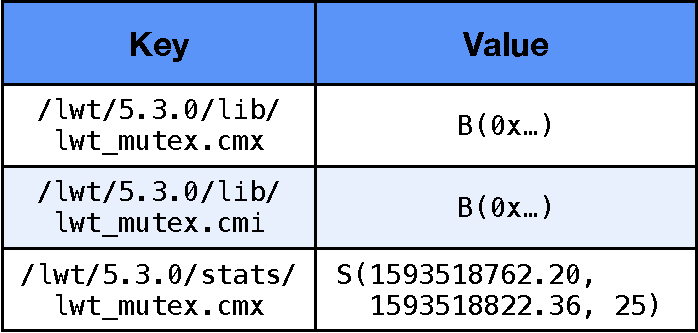
\includegraphics[scale=0.45]{figures/buildcache}
	\caption{A slice of the build cache key-value store.}
	\label{fig:buildcache}
	\vspace{-2.0cm}
\end{wrapfigure}
The value is either a binary artefact or a statistics triple.
Figure~\ref{fig:buildcache} shows the slice of the build cache key-value store.
The cache stores the artefacts (|cmx| and |cmi| files) produced as a result of
compiling the source file |lwt_mutex.ml| from the package |lwt| version
|5.3.0|. The build cache also stores the statistics for every artefact. The
example shows that the |lwt_mutex.cmx| was accessed 25 times. When several
developers and/or CI pipelines are running concurrently on different hosts,
they may attempt to add the same artefact to the store, or, if the artefact is
already present, retrieve it from the cache and update the corresponding
artefact statistics. It would be unwise to synchronize across all of the hosts
for updating the store, and suffer the latency hit and potential
unavailability. Hence, \name only writes an update to one of the replicas. The
replicas asynchronously share the updates between each other, and resolve
conflicting updates using used-defined three-way merge function. The merge
function for the build cache is given below.

\begin{lstlisting}[language=caml, numbers=left]
let merge (lca: value option) (v1: value) (v2: value) : value =
  match lca, v1, v2 with
  | None, B a1, B a2 (* no lca *)
  | Some (B _), B a1, B a2 -> assert (a1 = a2); B a1
  | None, S(c1,la1,h1), S(c2,la2,h2) -> (* no lca *)
      S(min c1 c2, max la1 la2, h1 + h2)
  | Some(S(_,_,h0)), S(c1,la1,h1), S(c2,la2,h2)->
      S(min c1 c2, max la1 la2, h1 + h2 - h0)
  | _ -> failwith "impossible"
\end{lstlisting}

The key idea here is that \name tracks the \emph{causal history} of the state
updates such that it is always known what the \emph{lowest common ancestor}
(LCA) state is, if one exists. This idea is analogous to how Git tracks history
with the notion of \emph{branches}. The merge function is applied to the LCA
and the two conflicting versions to determine the new state. In the case of
build cache, since the builds are reproducible, the binary artefacts will be
the same (line 4). The only interesting conflicts are in the statistics. The
merge function picks the earliest creation timestamp, latest last accessed
timestamp, and the sum of the new cache hits since the LCA in the two branches
and the original value at the LCA, if present (lines 5--8).

\begin{wrapfigure}{r}{0.5\textwidth}
	\vspace{-0.9cm}
	\centering
	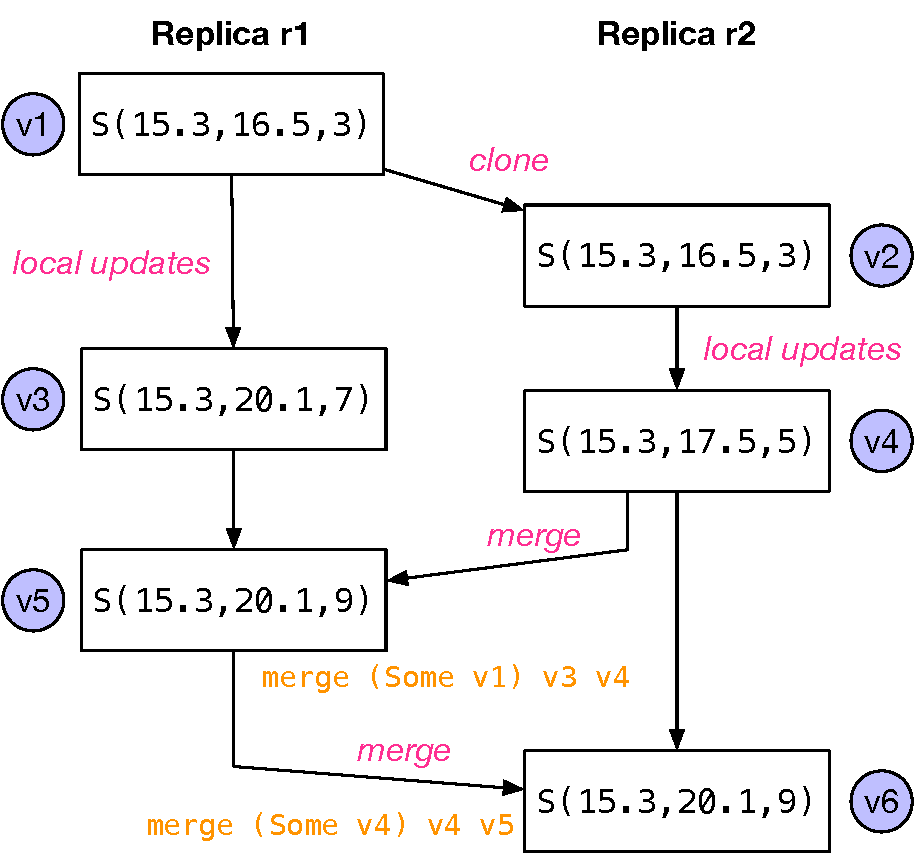
\includegraphics[scale=0.4]{figures/replica_merge}
	\caption{Merging conflicting statistics updates.}
	\label{fig:replica_merge}
	\vspace{-0.8cm}
\end{wrapfigure}
Figure~\ref{fig:replica_merge} shows how the merge function helps reconcile
conflicts. The arrows capture the happens-before relationship between the
states. Assume that replica |r2| starts off by cloning the branch corresponding
to replica |r1|. Subsequently both |r1| and |r2| performed local updates. The
remote updates are reconciled by calling the merge function on each of the
conflicting values. The value |v5| is obtained with merging the values |v3| and
|v4| with |v1| as LCA. Importantly, observe that the cache hit count is |9| in
|v5| which corresponds to the sum of |3| hits in the initial state, |4|
additional hits in |r1| and |2| additional hits in |r2|. At this point, |r1|
has all the changes from |r2|, but the vice-versa is not true. Subsequently,
when |r1| is merged into |r2|, both the replicas have converged.

\begin{figure}%{r}{0.6\textwidth}
	\vspace{-0.5cm}
	\begin{lstlisting}
let compile s (* session *) =
	let ts = Unix.gettimeofday () in
	let lib = ["lwt";"5.3.0";"lib"] in
	let stats = ["lwt";"5.3.0";"stats"] in
	refresh s >>= fun () ->
	read s (lib @ ["lwt_mutex.cmx"]) >>= fun v ->
	match v with
	| None ->
			let (cmx, cmi, o) = ocamlopt "lwt_mutex.ml" in
			write s (lib @ ["lwt_mtex.cmx"]) (B cmx) >>= fun _ ->
			write s (stats @ ["lwt_mutex.cmx"]) (S (ts,ts,0)) >>= fun _ ->
			... (* similarly for cmi and o files *)
			publish s >>= fun _ ->
			return (cmx, cmi, o)
	| Some cmx ->
			read s (stats @ ["lwt_mutex.cmx"]) >>= fun (Some M(c,la,h)) ->
			write s (stats @ ["lwt_mutex.cmx"]) (S (c,ts,h+1)) >>= fun _ ->
			read s (lib @ ["lwt_mutex.cmi"]) >>= fun (Some cmi) ->
			read s (lib @ ["lwt_mutex.o"]) >>= fun (Some o) ->
			... (* update stats for cmi and o file *)
			publish s >>= fun _ ->
			return (cmx, cmi, o)
	\end{lstlisting}
	\caption{Compiling \texttt{lwt\_mutex.ml}.}
	\label{code:compile}
	\vspace{-1cm}
\end{figure}

\subsection{Transactions}

Now that we the mergeable value type for the build cache, let us see how we can
compile |lwt_mutex.ml| using \name. Figure~\ref{code:compile} shows the code
for compiling |lwt_mutex.ml|. In \name, the clients interact with the store in
\emph{isolated} sessions. A session can fetch recent updates using the
|refresh| primitive and make \emph{all} the local updates visible to other
sessions using the |publish| primitive. During |refresh|, any conflicting
updates are resolved using the three-way merge function associated with the
value type.

In order to compile |lwt_mutex.ml|, we first refresh the session to get any
recent updates. Then, we check whether the |lwt_mutex.cmx| file is in the build
cache. If not, the source file is compiled, and the resultant artefacts (|cmx|,
|cmi|, |o| files) and the corresponding entries for updated statistics are
written to the store. Finally, the all the local updates are published.

The all or nothing property of |refresh| and |publish| is critical for the
correctness of this code. Observe that when the artefact is locally compiled,
all the artefacts and their statistics are published atomically. This ensures
that if a session sees the |cmx| file, then other artefacts and their
statistics will also be visible. Thus, \name makes it easy to write highly-available,
complex distributed applications in an idiomatic fashion.


%%%%%%%%%%%%%%%%%%%%%%%%%%%%%%%%%%%%%%%%%%%%%%%%%%
%Programming model.
\clearemptydoublepage
%\pagenumbering{arabic}

\chapter{Programming Model}
\label{chap:prog_model}
\begin{wrapfigure}{r}{0.6\textwidth}
	\vspace{-1.3cm}
	\centering
	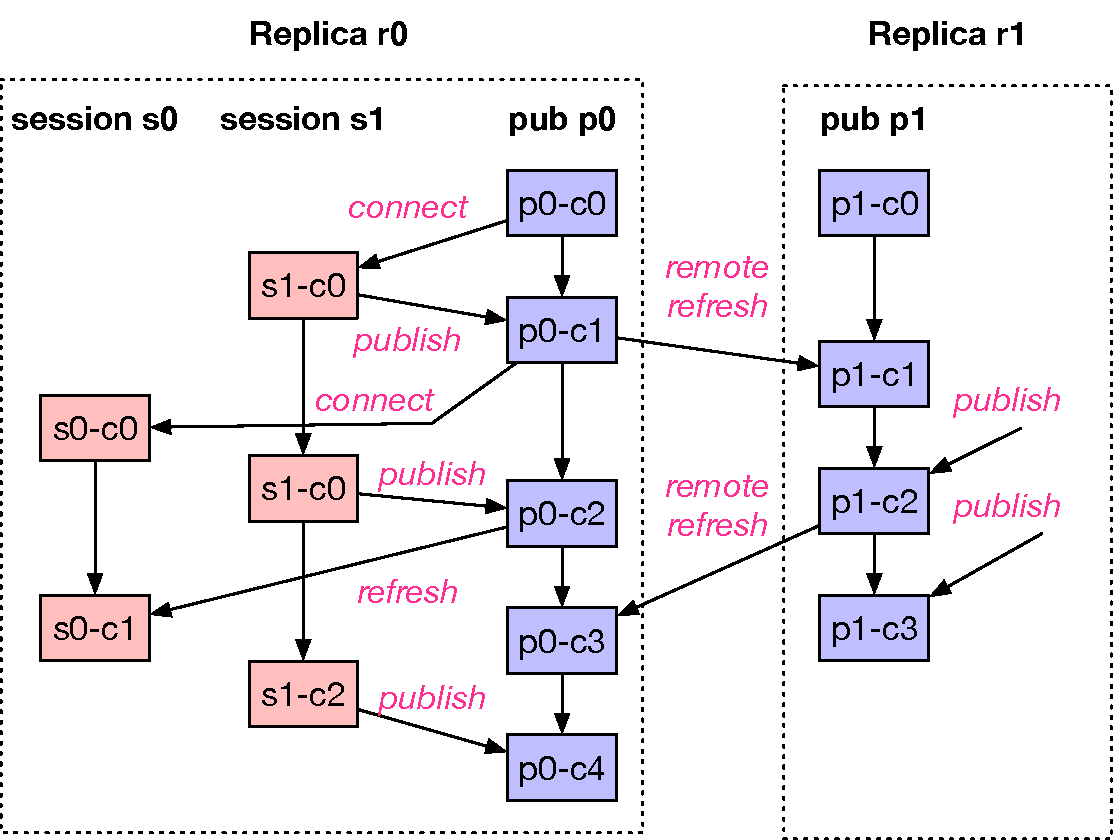
\includegraphics[scale=0.35]{figures/session_merge}
	\caption{\name system and programming model.}
	\vspace{-0.5cm}
	\label{fig:session_merge}
\end{wrapfigure}
In this section, we shall describe the system and programming model of \name
from the developers point-of-view. The \name store consists of several
replicas, which are fully or partially replicated~\cite{Crain15}. The replicas
asynchronously distribute updates amongst themselves until they converge. The
key property that enables \name to support mergeable types and isolated
transactions is that \name tracks the history of the store in the same way that
Git tracks the history of a repository.

Figure~\ref{fig:session_merge} presents the schematic diagram of the system and
programming model. Each replica has a distinguished public branch |pub|, which
records the history of the changing state at that replica. Each node in this
connected history graph represents a \emph{commit}. Whenever a new client
connection is established, a new branch is forked off the latest commit in the
public branch. Any reads or writes in this session is only committed to this
branch unless explicitly published. This ensures the isolation property of each
session. The figure shows the creation of two session in the replica |r0|.

The simplified \name API is given below:

\begin{lstlisting}
type config  (* Store configuration *)
type session
type key = string list
type value   (* Type of mergeable values in the store *)

val connect : config -> session Lwt.t
val close   : session -> unit Lwt.t
val read    : session -> key -> value option Lwt.t
val write   : session -> key -> value -> unit Lwt.t
val publish : session -> unit Lwt.t
val refresh : session -> unit Lwt.t
\end{lstlisting}

When a client connects to a \name store, a new session is created, which is
rooted to one of the replicas in the store. Every write creates a commit in the
session performing the write. As previously explained, \name permits the
sessions to atomically |publish| their updates and |refresh| to obtain latest
updates. The |publish| operation squashes all the local commits since the
previous |refresh| or |publish| to a single commit, and then \emph{pushes} the
changes to the public branch on the replica to which the session is rooted. The
|refresh| operation \emph{pulls} updates from the public branch into the
current sessions branch. Both |publish| and |refresh| may invoke the merge
function on the value type if there are conflicts. The objects that written to
each replica are asynchronously replicated to other replicas. \name offers
causal consistency for operations on each key.

Periodically, the changes from other public branches are \emph{pulled} into a
replica's public branch (remote refresh). This operation happens
\emph{implicitly} and asynchronously, and does not block the client on that
replica. When a session is closed, the outstanding writes are implicitly
published. Similarly, when a session is connected, there is an implicit refresh
operation.

Observe that both the local and the remote refresh operations are non-blocking
-- it is always safe for |refresh| to return with updates only from a subset of
public branches. The only push operation is due to |publish|. When pushing to a
branch, it is necessary to atomically update the target branch to avoid
concurrency errors. The key observation is that only the session that belongs
to a replica can push to the public branch on that replica. This can be
achieved with replica-local concurrency control and does not require
coordination among the replicas. Hence, \name transactions do not need
inter-replica coordination, and hence, are available.

When a particular replica goes down, the sessions that are rooted to that
replica may not have enough history to be able to |refresh| and |publish| to
other replicas. In particular, since |refresh| and |publish| will need to
discover the LCA in the case of conflicting updates. Since the objects are
asynchronously replicated across the replicas, the recent writes to the replica
that went down may not have been replicated to other replicas. Hence, \name
requires sticky availability~\cite{Bailis13} -- the sessions need to reach the
logical replica to which it originally connected. In practice, with partial
replication, a logical replica may be represented by a set of physical servers.
As long as one of these physical servers is reachable, the system remains
available for that session.

Compared to traditional transactions usually executed at a particular isolation
level, |refresh| and |publish| permits more fine-grained, explicit control of
visibility. In \name, transactions are delimited by |publish| operations, begin
and end of sessions. For example, the set of writes performed between
consecutive |publish| operations are made visible atomically outside the
session. The transaction may abort if the three-way merge function throws an
exception. However, in practice, the useful MRDTs are designed in such a way
that a merge is always possible, and the failure of the merge function
represents a bug. This idea of merge always being possible ensures \emph{strong
eventual consistency}, espoused by convergent replicated data
types~\cite{Shapiro11}. \name adds transactional support over strong eventual
consistency.

The |publish| and |refresh| can be used to achieve well-known isolation levels.
For example, snapshot isolation~\cite{Berenson95} is achieved by |refresh|ing
at that beginning of the transaction and |publish|ing at the end of the
transaction with no intervening |refresh|es. Unlike snapshot isolation, the
conflicting updates will be resolved with the three-way merge function. If two
consecutive |publish| operations are interspersed with |refresh|es, then one
gets the monotonic atomic view~\cite{Bailis13} isolation level.


%%%%%%%%%%%%%%%%%%%%%%%%%%%%%%%%%%%%%%%%%%%%%%%%%%

%Implementation
\clearemptydoublepage
%\pagenumbering{arabic}

\chapter{Implementation}
\label{chap:implementation}
In this section, we describe the instantiation of \name on
Cassandra~\cite{Cassandra}, a popular, industrial-strength, column-oriented,
distributed database. Cassandra offers eventual consistency with a
last-write-wins conflict resolution policy. Cassandra also offers complex data
types such as \texttt{list}, \texttt{set} and \texttt{map} with baked-in conflict resolution policies. Given the
richness of replicated data types, the available complex data types are quite
limiting. Cassandra also offers lightweight transactions (distributed
compare-and-update) implemented using the Paxos consensus
protocol~\cite{lamport2001paxos}. Lightweight transactions are limited to operate
on only one object. \name does not use lightweight transactions since their cost is prohibitively high due to consensus. As
mentioned previously \name only requires sticky availability, and so uses a
replica-local lock for ensuring mutual exclusion when multiple sessions try to
update the public branch on a replica concurrently.

By instantiating \name on Cassandra, we offload the concerns of replication,
fault tolerance, availability and convergence to the backing store. On top of
Cassandra, \name uses Irmin~\cite{Irmin}, an OCaml library for persistent
stores with built-in branching, merging and reverting facilities. Irmin can be
configured to use different storage backends, and in our case, the storage is
Cassandra. Importantly, Cassandra being a distributed database serves the
purpose of the networking layer in addition to persistent storage. While Irmin permits
arbitrary branching and merging, \name is a specific workflow on top of Irmin
which retains high availability.

\subsection{Irmin data model}

\begin{wrapfigure}{r}{0.5\textwidth}
	\vspace{-1.6cm}
	\centering
	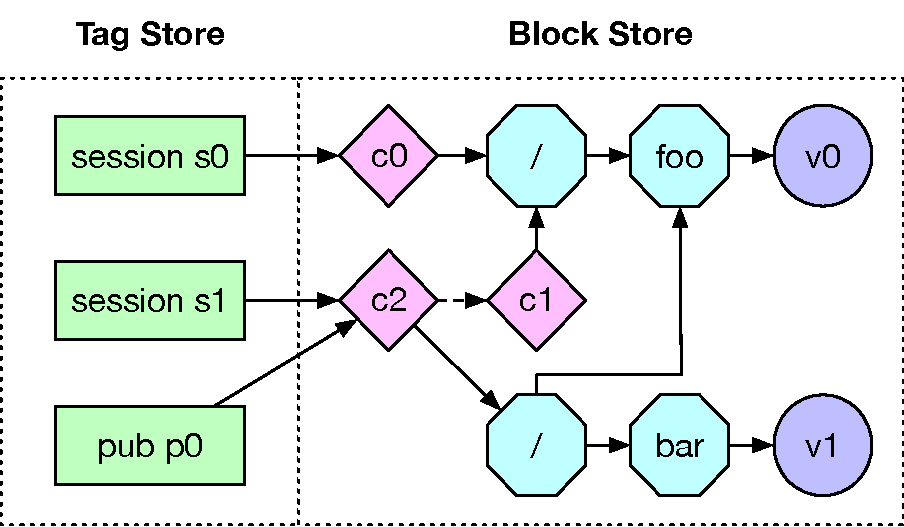
\includegraphics[scale=0.4]{figures/irmin_store}
	\caption{A sample Irmin store. The rectangles are tags, diamonds are commit
	objects, octagons are tree object, and circles are blob objects.}
	\vspace{-0.8cm}
	\label{fig:irmin_store}
\end{wrapfigure}
The expressivity of Irmin imposes significant burden on the underlying storage.
For efficiently storing different versions of the state as the store evolves,
Irmin uses the Git object model. Figure~\ref{fig:irmin_store} shows a snapshot
of the state of the Irmin store. There are two kinds of stores: a mutable tag
store and an immutable, content-addressed block store. The tag store records
the branches and the commit that corresponds to this branch. In this example,
we have three branches, |session s0|, |session s1| and |pub p0|.

The block store is content-addressed and has three different kinds of objects:
commits, tree and blobs. A commit object represents a commit, and it may have
several parent commits and a single reference to a tree node. For example, the
commit |c2|'s parent is |c1|, and |c0| and |c1| do not have any parent commits.
The tree object corresponds to directory entries in a filesystem, and
recursively refer to other tree objects or a blob object. Unlike Git, Irmin
allows blob objects to be arbitrary values, not just files. The blob objects
may refer to other blob objects. In the session |s1|, reading the keys
|["foo"]| and |["bar"]| would yield |Some v0| and |Some v1|, respectively.

Observe that all the commits share the tree object |foo| and its descendents,
thanks to the block store being content addressed. Content addressibility of
the block store means that as the store evolves, the contents of the store are
shared between multiple commits, if possible. On the other hand, updating a
value in a deep hierarchy of tree objects would necessitate allocating a new
spine in order to maintain both the old and the new versions. Thus, each write
in \name will turn into several writes to the underlying storage.

\subsection{Cassandra instantiation}

For instantiating \name on Cassandra, we use two tables, one for the tag store
and another for the block store. For the tag store, the key is a |string| (tag)
and the value is a |blob| (hash of the commit node). For the block store, the
key is a |blob| (hash of the content), and the value is a |blob| (content).
Irmin handles the logic necessary to serialize and deserialize the various Git
objects into binary |blob|s and back.

Cassandra replicates the writes to the tag and block tables asynchronously
amongst the replicas. Each replica periodically merges the public branches of
other replicas into its public branch to fetch remote updates. Due to eventual
consistency of Cassandra, it may be the case that not all the objects from a
remote replica are available locally. For example, the merge function may find
a new commit from a remote replica, but the tree object referenced by a commit
object may not available locally. In this situation, \name simply skips merging
this branch in this round. Cassandra ensures that eventually the remote tree
object will arrive at this replica and will be merged in a subsequent remote
refresh operation. Thus, fetching remote updates is a non-blocking operation.

In Irmin, the tag store is update with a compare-and-swap to ensure that
concurrent updates to the same tag should be disallowed. Naively implementing
this in Cassandra would necessitate the use of lightweight transactions and
suffer prohibitive costs. By restricting the \name programming model
(Section~\ref{sec:model}) such that entries in the tag store (in particular,
the tag corresponding to the public branch of the replica) is only updated on
that replica, we remove the necessity for lightweight transactions. Thus, we
do not depend on any special features of Cassandra to realise the \name model,
and \name can be instantiated on any eventually consistent key-value store.

\subsection{Recursive merges}
\label{sec:rec_merge}

A particular challenge in making \name scalable is the problem of recursive
merges. Consider a simple mergeable counter MRDT, whose implementation is:
\begin{lstlisting}
let merge lca v1 v2 =
let old = match lca with None -> 0 | Some v -> v in
v1 + v2 - old
\end{lstlisting}

\begin{wrapfigure}{r}{0.45\textwidth}
	\centering
	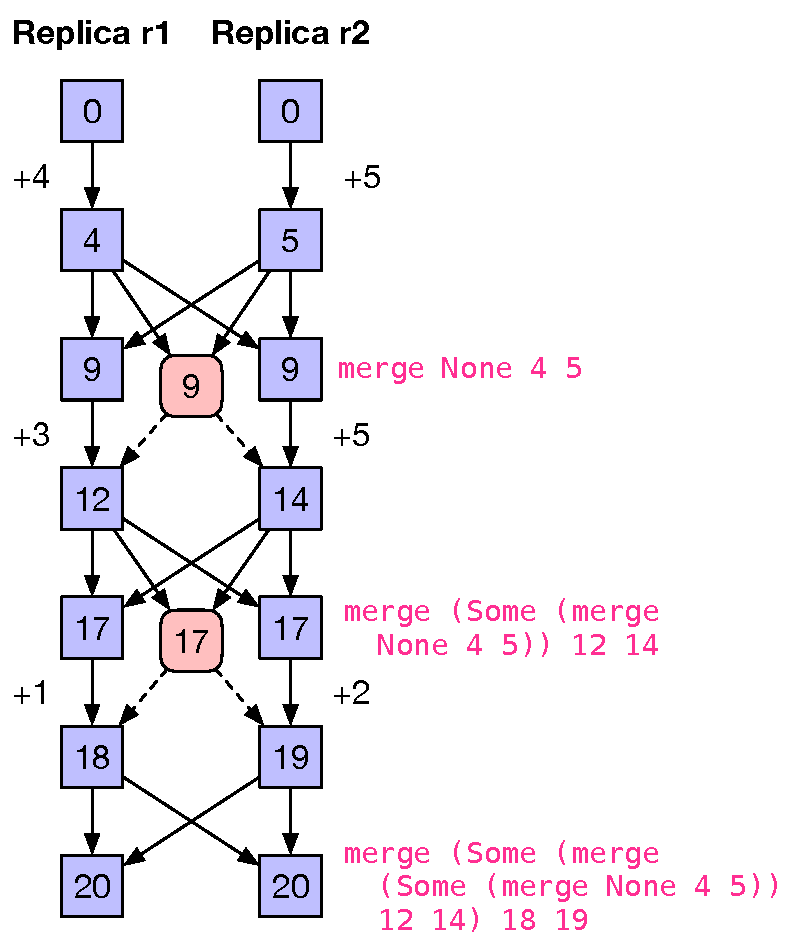
\includegraphics[scale=0.45]{figures/recursive}
	\caption{Recursive merge. Rounded rectangles are the results of recursive
		merges.}
	\label{fig:recursive}
	\vspace{-0.9cm}
\end{wrapfigure}
Consider the execution history presented in Figure~\ref{fig:recursive} which
shows the evolution of a single counter. The history only shows the interaction
between two replicas, and does not show any sessions. Each node in the history
is a commit. Since we want to focus on a single counter, for simplicity, we
ignore the tree nodes and the node labels show the counter value.

Initially the counters are |0|, and each replica concurrently increments the
counter by |4| and |5|. When the replicas perform remote refreshes, they invoke
|merge None 4 5| to resolve the conflict updates yielding |9|. The LCA is
|None| since there is no common ancestor.

Subsequently, the replicas increment the counters by |3| and |5|. Now, consider
that the replicas merge each other's branches. When merging |12| and |14|,
there are two equally valid LCAs |4| and |5|. Picking either one of them leads
to incorrect result. At this point, Irmin merges the two LCAs             using
|merge None 4 5| to yield |9|, which is used as the LCA for merging |12| and
|14|. This yields the value |17|. The result of merging the LCAs is represented
as a rounded rectangle. Importantly, the result of the recursive merge |9| is
not a parent commit of |12| and |14| (distinguished by the use of dotted
arrows). This is because the commit nodes are stored in the content-addressed
store, and adding a new parent to the commit node would create a distinct node,
whose hash is different from the original node. Any other nodes that referenced
the original commit node will continue to reference the old node. As a result,
the recursive merges will need to be performed again for subsequent requests!

Consider that the replicas further evolve by incrementing |1| and |2|, yielding
|18| and |19|. When these commits are merged on remote refresh, there are two
LCAs |12| and |14|, which need to be merged. This in turn has two LCAs |4| and
|5|, which need to be merged. Thus, every subsequent recursive merge, which is
very likely since the replicas merge each other's branches, requires repeating
all the previous recursive merges. This does not scale.

We solve this problem by having a separate table in Cassandra that acts as a
cache, recording the result of LCA merges. Whenever \name encounters a
recursive merge, the cache is first consulted before performing the merge. In
this example, when |18| and |19| are being merged, \name first checks whether
the two LCAs |12| and |14| are in the cache. They would not be. This triggers a
recursive merge of LCAs |4| and |5|, whose result is in the cache, and is
reused. The cache is also updated with an entry that records that the merge of
the LCAs |12| and |14| is the commit corresponding to |17|.

\subsection{Garbage collection}
\label{sec:gc}

While traditional database systems only store the most recent version of the
data, \name necessitates that previous versions of the data must also be kept
around for three-way merges. While persistence of prior
versions~\cite{Driscoll86,farinier15} is a useful property for audit and tamper
evidence, the \name API presented here does not provide a way to access earlier
versions. The question then is: when can those prior versions be garbage
collected?

We have not yet implemented the garbage collector for \name on Cassandra, but we
sketch the design here. Git is equipped with a garbage collector (GC) that
considers that any object in the block store that is reachable from the tag
store is alive. Unreachable objects are be deleted. Our aim is to assist the
Git-like GC by pruning the history graph of nodes which will no longer be used.
The key idea is that if a commit node will not be used for LCA computation,
then that commit node may be deleted. Deleting commit nodes will leave dangling
references from its referees, but Irmin can be extended to ignore
dangling references to commit nodes.

\begin{wrapfigure}{r}{0.5\textwidth}
	\vspace{-1cm}
	\centering
	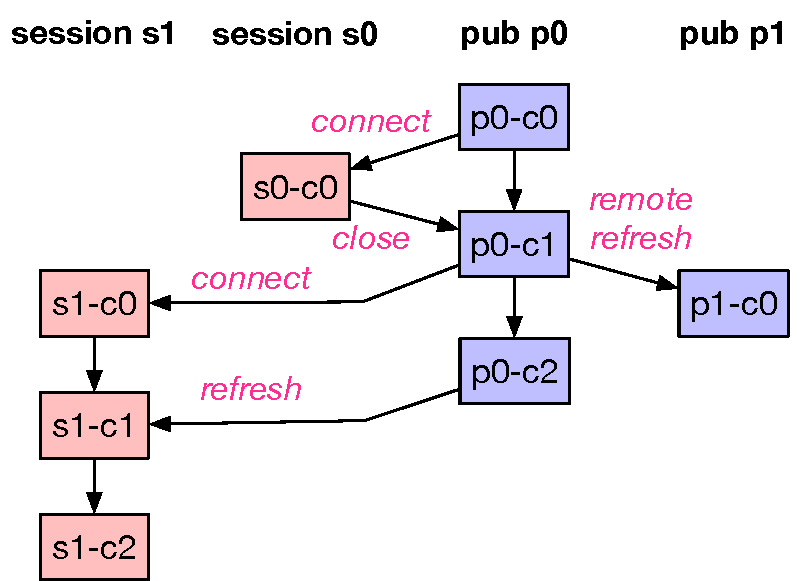
\includegraphics[scale=0.45]{figures/gc}
	\caption{Garbage collection. Here, the commits \texttt{p0-c0} and
		\texttt{s0-c0} may be deleted.}
	\label{fig:gc}
	\vspace{-0.7cm}
\end{wrapfigure}
For individual sessions, once the session is closed, the corresponding entry in
the tag store, and all the commits by that session may be deleted. In the
execution history in Figure~\ref{fig:gc}, the commit node |s0-c0| may be
deleted. The next question is when can commits on public branch be deleted. For
each ongoing session in a replica, we maintain the latest commit in the public
branch against which |refresh| was performed. The earliest of such commits in
the public branch and its descendants must be retained, since they are
necessary for the three-way merge. For example, in Figure~\ref{fig:gc}, session
|s1| refreshed against |p0-c2|, and |s1| is the only ongoing session. If |s1|
publishes, then |p0-c2| will be the LCA commit.

A similar reasoning is used for remote refreshes. When a commit in the public
branch of a replica has been merged into the public branches of all the other
replicas, then the ancestors of such commits will not be accessed and can be
deleted. In Figure~\ref{fig:gc}, assume that we only have two replicas. Since
|p0-c1| was merged by the public branch |p1|, |p0-c1| will be the LCA commit
for subsequent remote refreshes by |p1|. Given that |p0-c0| is neither
necessary for remote refreshes nor for ongoing sessions, |p0-c0| can be
deleted.


%%%%%%%%%%%%%%%%%%%%%%%%%%%%%%%%%%%%%%%%%%%%%%%%%%

%Evaluation
\clearemptydoublepage
%\pagenumbering{arabic}

\chapter{Evaluation}
\label{chap:evaluation}
In this section, we evaluate the performance of \name instantiation on
Cassandra. Our goal is to assess the suitability of \name for programming
loosely connected distributed applications. To this end, we first quantify the
overheads of implementing \name over Cassandra. Subsequently, we assess the
performance of MRDTs implemented using \name. And finally, we study the
performance of distributed build cache (Section~\ref{sec:motivation}).

\subsection{Experimental setup}

For the experiments, we use a Cassandra cluster with 4 nodes within the same
data center. Each Cassandra node runs on a baremetal Intel\textregistered
Xeon\textregistered E3-1240 CPU, with 4 physical cores, and 2 hardware threads
per core. Each core runs at 3.70GHz and has 128KB of L1 data cache, 128KB of L1
instruction cache, 1MB L2 cache and 8MB of L3 cache. Each machine has 32GB of
main memory. The machines are unloaded except for the Cassandra node. The ping
latency between the machines is 0.5ms on average. The clients are run on a
machine with the same configuration in the same data center.

For the experiments, Cassandra cluster is configured with a replication factor
of 1, read and write consistency levels of |ONE|. Hence, the cluster maintains
a single copy of each data item, and only waits for one of the servers to
respond to return the result of read and write to the client. These choices
lead to eventual consistency where the reads may not return the latest write.
The cluster may be configured with larger replication factor for better fault
tolerance. However, stronger consistency levels are not useful since \name
enforces per-key causal consistency over the underlying eventual consistency
offered by Cassandra. In fact, choosing strong consistency for reads and writes
in Cassandra does not offer strong consistency in \name since the visibility of
updates in \name is explicitly controlled with the use of |refresh| and
|publish|.

\subsection{Baseline overheads}

\begin{wrapfigure}{r}{0.55\textwidth}
	\vspace{-1cm}
	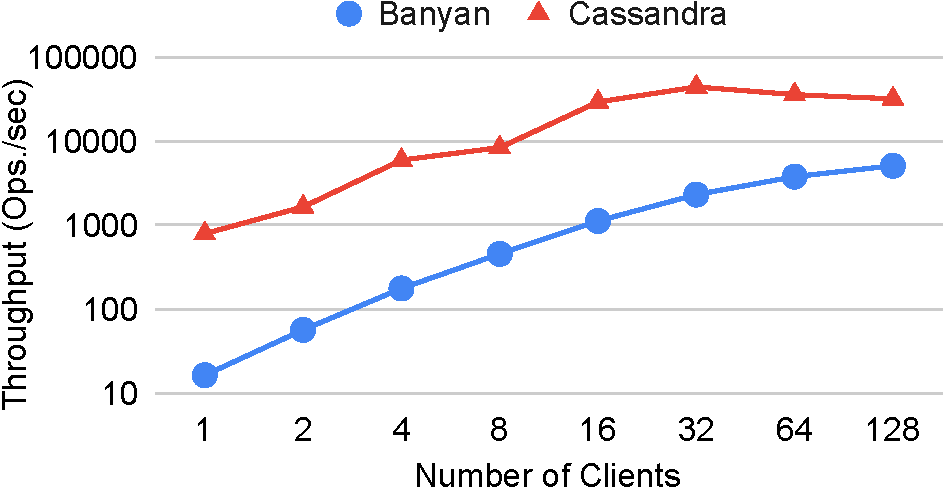
\includegraphics[scale=0.40]{results/baseline}
	\caption{Performance comparison between \name and Cassandra on LWW string
	value.}
	\label{res:baseline}
	\vspace{-0.5cm}
\end{wrapfigure}
Given that \name has to persist every version of the store, what is the impact
of \name when compared to using Cassandra in a scenario where Cassandra would
be sufficient? We measure the throughput of performing 32k operations, with
80\% reads and 20\% writes with different numbers of clients. The keys and
values are 8 and 128 byte strings, respectively. For \name, we use
last-writer-wins resolution policy, which is the policy used by Cassandra. The
results are presented in Figure~\ref{res:baseline}.

With 1 client, \name performs 16 operations per second, while Cassandra
performs 795 operations per second. Cassandra offers 50$\times$ more throughput
than \name with 1 client. This is due to the fact that every read (write)
performs 4 reads (3 reads and 4 writes) to the underlying store to create and
access the tag, commit and tree nodes. \name additionally includes marshalling
and hashing overheads for accessing the content-addressed block store.
Cassandra does not include any of these overheads. Luckily, \name overheads are
local to a client, and hence, can be easily parallelized. With 1 client, the
cluster is severely under utilized, and the client overheads dominate. With
increasing number of clients, the cluster is better utilized. At 128 clients,
Cassandra performs 31274 operations per second where as \name performs 5131
operations per second, which is a slowdown of 6.2$\times$. We believe that
these are reasonable overheads given the stronger consistency and isolation
guarantees, and better programming model offered by \name.

At the end of 32k operations, Cassandra uses 4.9MB of disk space, while \name
uses 1.8GB of disk space. As mentioned earlier (\S\ref{sec:gc}), we have yet to implement garbage collection for
\name -- once implemented, we expect this space usage will come down significantly.

\subsection{Mergeable Types}

\paragraph*{\textbf{Counter}} We begin with the counter data type discussed in
Section~\ref{sec:rec_merge}. How does \name counter perform on when
concurrently updated by multiple clients? For the experiment, the value type is
a counter that supports increment, decrement and read operations. The clients
perform 32k increment or decrement operations on a key randomly selected from a
small key space. Each client refreshes and publishes after every 100
operations. By choosing a small key space, we aim to study the scalability of
the system with large number of conflicts.

\begin{wrapfigure}{r}{0.55\textwidth}
	\vspace{-0.5cm}
	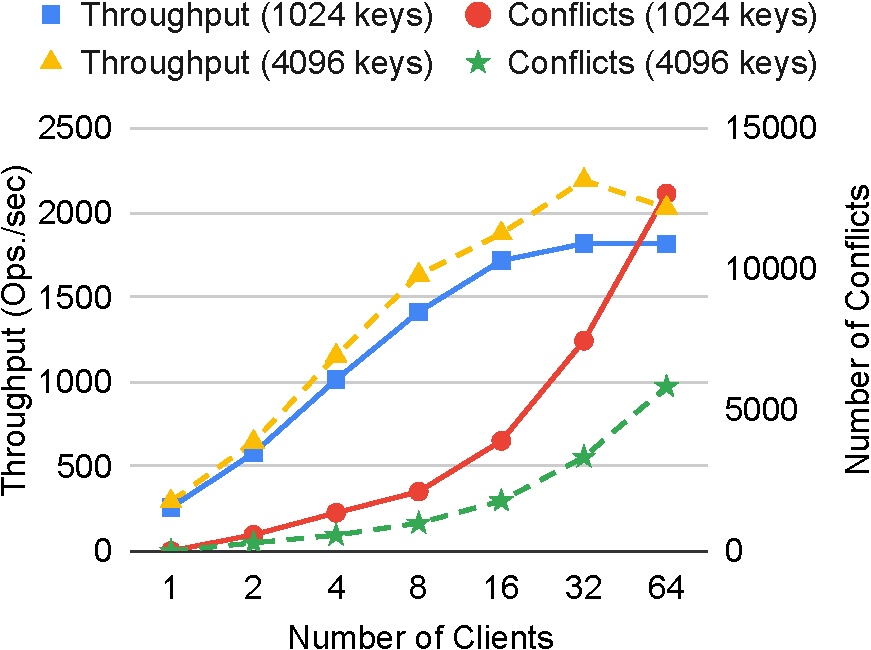
\includegraphics[scale=0.45]{results/counter}
	\caption{Performance of counter MRDT.}
	\label{res:counter}
	\vspace{-0.5cm}
\end{wrapfigure}
Figure~\ref{res:counter} shows the performance result for two key spaces of
size 1024 and 4096 keys. With 1 client, there are no conflicts. The conflicts
increases with increasing number of clients. We get a peak throughput of 1814
(2027) operations per second with a key space of 1024 (4096) keys. Observe that
the number of conflicts is considerably lower with 4096 keys when compared to
1024 keys. As a result, the throughput is higher with 4096 keys. The result
shows that the throughput of the system is proportional to the number of
conflicting operations.

\paragraph*{\textbf{Blob log}} Another useful class of MRDTs are
\emph{mergeable logs}, where each log message is a string. Such a distributed
log is useful for collecting logs in a distributed system, and examining the
logs in their global time order. To this end, each log entry is a pair of
timestamp and message, and the log itself is a list of such entries in reverse
chronological order. The merge function for the mergeable log extracts the
newer log entries from both the versions, sorts the newer entries in reverse
chronological order and returns the list obtained by appending the sorted newer
entries to the front of the log at the LCA.

While this implementation is simple, it does not scale well. In particular,
each commit stores the entire log as a single serialized blob. This does not
take advantage of the fact that every commit can share the tail of the log with
its predecessor. Moreover, every append to the log needs to deserialize the
entire log, append the new entry and serialize the log again. Hence, append is
an $O(n)$ operation, where $n$ is the size of the log. Merges are also worst
case $O(n)$. This is undesirable. We call this implementation a \emph{blob
log}.

\paragraph*{\textbf{Linked log}} We can implement a efficient logs by taking
advantage of the fact that every commit shares the tail of the log with its
predecessor. The value type in this log is:

\begin{lstlisting}
type value =
  | L of float (* timestamp *) * string (* message *)
	     * blob (* hash of prev value *)
	| M of blob list (* hashes of the values being merged *)
\end{lstlisting}

\begin{wrapfigure}{r}{0.4\textwidth}
	\vspace{-1cm}
	\centering
	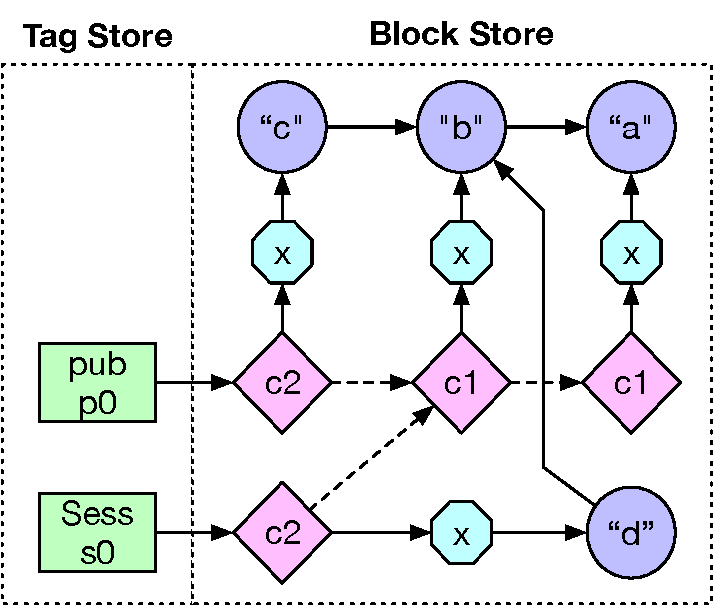
\includegraphics[scale=0.4]{figures/linked_log}
	\caption{A snapshot of linked log storage.}
	\label{fig:linked_log}
	\vspace{-0.5cm}
\end{wrapfigure}
The value is either a log entry |L(t,m,h)| with timestamp |t|, message |m| and
a hash of the previous value |h|. Appending to the log only needs to add a new
object that refers to the previous log value. Hence, append is $O(1)$.
Figure~\ref{fig:linked_log} shows a snapshot of the log assuming a single key
|x|. The log at |x| in the public branch |p0| (session |s0|) is |[a;b;c]|
(|[a;b;d]|). The merge operation simply adds a new value |M [h1;h2]|, which
refers to the hashes of the two log values being merged. This operation is also
$O(1)$. The read function for the log does the heavy-lifting of reading the log
in reverse chronological order.

\begin{wrapfigure}{l}{0.55\textwidth}
	\vspace{-0.5cm}
	\centering
	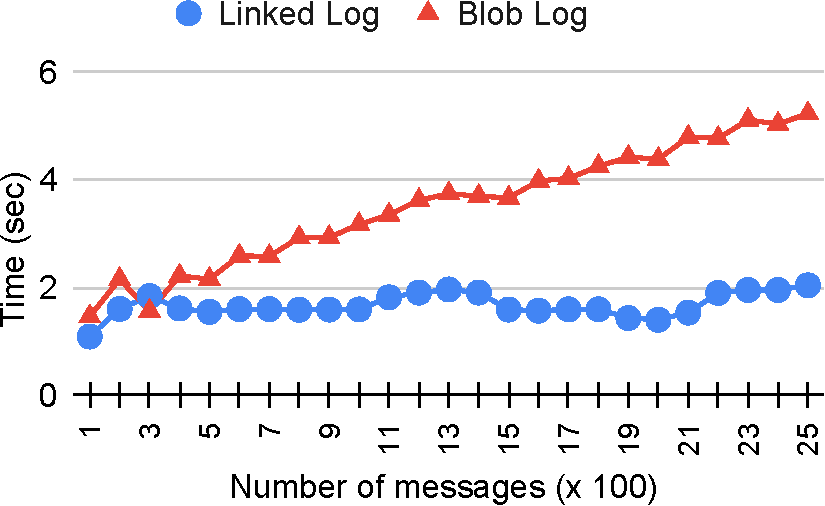
\includegraphics[scale=0.45]{results/log}
	\caption{Performance of mergeable logs.}
	\label{res:log}
	\vspace{-1.5cm}
\end{wrapfigure}
Observe that unlike the examples seen so far where the values do not refer to
other values, this \emph{linked log} implementation refers to other values as
heap data structures would do. Figure~\ref{res:log} shows the time taken to add
100 additional messages to the log with 4 clients. Observe that the time stays
constant with linked log but increases linearly with blob log. By being able to
share objects across different commits (versions), \name leads to efficient
implementations of useful data structures.

\subsection{Distributed build cache}

\begin{wrapfigure}{r}{0.45\textwidth}
	\vspace{-1cm}
	\centering
	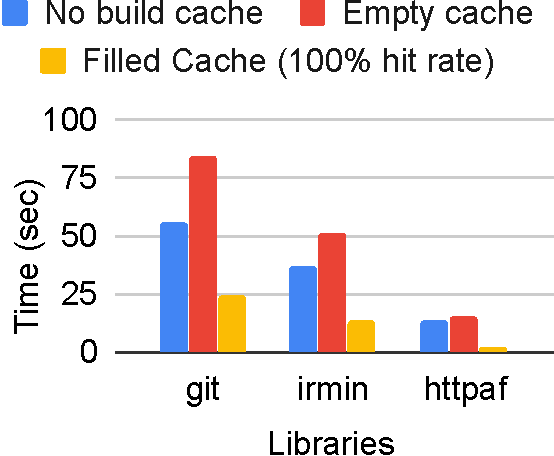
\includegraphics[scale=0.5]{results/build1}
	\caption{Performance of complete reuse of build artefacts.}
	\label{res:build1}
	\vspace{-0.5cm}
\end{wrapfigure}
In this section, we evaluate the performance of distributed build cache
described in Section~\ref{sec:motivation}. We have chosen three OCaml packages:
|git|, |irmin| and |httpaf| with common dependent packages. In the first
experiment, we measure the benefit of building a package that has already been
built in another workspace. Hence, the package artefacts will already be in the
build cache.

For each library, we measure the
baseline build time (1) without using the build cache, (2) using an empty build
cache, and (3) building the same package on a machine with the same package
having built earlier on a different machine. Figure~\ref{res:build1} shows the
results. We see that case using an empty build cache is slower than not using
the cache since the artefacts are stored in the cache. We also see that
building the same package on a different machine is faster due to the build
cache when compared to the baseline.

\begin{wrapfigure}{l}{0.45\textwidth}
	\vspace{-0.5cm}
	\centering
	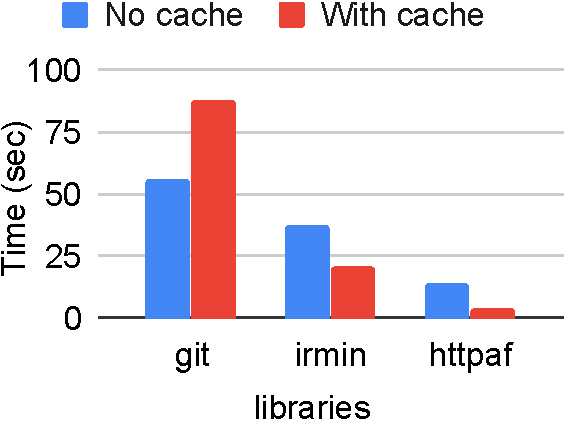
\includegraphics[scale=0.5]{results/build2}
	\caption{Performance of partial reuse of build artefacts.}
	\label{res:build2}
	\vspace{-0.5cm}
\end{wrapfigure}
A more realistic scenario is partial sharing of artefacts, where some of the
dependencies are in the cache and other need to be build locally, and added to
the cache. In this experiment, |git| package is first build on a machine with
an empty cache. Subsequently, |irmin| package is built on a second machine
(which will now benefit from the common artefacts in the cache). And finally,
building |httpaf| on a third machine, which benefits from both of the builds.
Figure~\ref{res:build2} shows the results. As expected, the |git| package build
is slower with cache than without since the cache is empty and the artefacts
need to be written to the cache additionally. Subsequent package builds benefit
from partial sharing of build artefacts. The results illustrate that \name not
only makes it easy to build complex applications like distributed build caches,
but the implementation also performs well under realistic workloads.


%%%%%%%%%%%%%%%%%%%%%%%%%%%%%%%%%%%%%%%%%%%%%%%%%%

%Related Work
\clearemptydoublepage
%\pagenumbering{arabic}

\chapter{Related Work}
\label{chap:related_work}
Several prior works have addressed the challenge of balancing the
programmability and performance under eventual consistency. RedBlue
consistency~\cite{Li12} offers causal consistency by default (blue), but
operations that require strong consistency (red) are executed in single total
order. Quelea~\cite{Sivaramakrishnan15} and MixT~\cite{Milano18} offer
automated analysis for classifying and executing operations are different
consistency levels embedded in weakly isolated transactions, paying the cost of
proportional to the consistency level. Indeed, mixing weaker consistency and
transactions have been well-studied~\cite{Brutschy17,Kraska13,CosmosDB}.

\name only supports causal consistency, but it is known to be the strongest
consistency level that remains available~\cite{Llyod11}. While prior works
attempt to reconcile traditional isolation levels with weak consistency, \name
leaves the choice of reading and writing updates to and from other transactions
to the client through the use of |publish| and |refresh|. We believe that
traditional database isolation levels are already quite difficult to get
right~\cite{Kaki17}, and attempting to provide a fixed set of poorly understood
isolation levels under weak consistency will lead to proliferation of bugs.

\name is distinguished by the equipping data types with the ability to handle
conflicts (three-way merge functions). \name builds on top of
Irmin~\cite{Irmin} library. Irmin allows arbitrary branching and merging
between different branches at the cost of having to expose the branch name.
\name refreshes and publishes implicitly to the public branch at a repository,
which obviates the need for naming branches explicitly. Irmin does not include
a distribution and convergence layer; \name uses Cassandra for this purpose.
\name provides causal consistency and coordination free transactions over
weakly consistent Cassandra. Several prior work have similarly obtained
stronger guarantees weaker stores~\cite{Sivaramakrishnan15,Bailis13b}.

TARDiS~\cite{Crooks16} supports user-defined data types, and a transaction
model similar to \name. TARDiS is however a machine model that exposes the
details of explicit branches and merges to the developer, whereas \name is a
programming model that can be instantiated on any eventually consistent
key-value store. For instance, in TARDiS programmers need to invoke a separate
merge transaction that does an n-way merge. \name transaction model is more
flexible than TARDiS. For example, \name can support monotonic atomic view,
which TARDiS cannot -- TARDiS transactions do not have a way of allowing more
recent updates since the transaction began. TARDiS does not discuss merges
without LCAs or the issue with recursive merges. We found recursive merges to
be a very common occurrence in practice. Concurrent
revisions~\cite{Burckhardt12} describe a programming model with branch and
merge workflow with explicit branches and restrictions on the shape of history
graphs. \name makes the choice of branches to publish and refresh implicit
leading to a simpler model. Concurrent revisions does not include an
implementation.


%%%%%%%%%%%%%%%%%%%%%%%%%%%%%%%%%%%%%%%%%%%%%%%%%%

%Conclusion
\clearemptydoublepage
%\pagenumbering{arabic}

\chapter{Conclusion}
\label{chap:conclusion}
\section{Conclusion}
\label{sec:conc}

We present \name, a novel programming model for developing loosely connected
distributed applications based on the principles of Git. We illustrate the
practicality of this approach by instantiating \name on Cassandra, an
off-the-shelf eventually consistent distributed store. Our experimental results
suggests that \name makes it easy to build complex distributed applications
without compromising performance.

%%%%%%%%%%%%%%%%%%%%%%%%%%%%%%%%%%%%%%%%%%%%%%%%%%


%In this section, we describe the instantiation of \name on
Cassandra~\cite{Cassandra}, a popular, industrial-strength, column-oriented,
distributed database. Cassandra offers eventual consistency with a
last-write-wins conflict resolution policy. Cassandra also offers complex data
types such as \texttt{list}, \texttt{set} and \texttt{map} with baked-in conflict resolution policies. Given the
richness of replicated data types, the available complex data types are quite
limiting. Cassandra also offers lightweight transactions (distributed
compare-and-update) implemented using the Paxos consensus
protocol~\cite{lamport2001paxos}. Lightweight transactions are limited to operate
on only one object. \name does not use lightweight transactions since their cost is prohibitively high due to consensus. As
mentioned previously \name only requires sticky availability, and so uses a
replica-local lock for ensuring mutual exclusion when multiple sessions try to
update the public branch on a replica concurrently.

By instantiating \name on Cassandra, we offload the concerns of replication,
fault tolerance, availability and convergence to the backing store. On top of
Cassandra, \name uses Irmin~\cite{Irmin}, an OCaml library for persistent
stores with built-in branching, merging and reverting facilities. Irmin can be
configured to use different storage backends, and in our case, the storage is
Cassandra. Importantly, Cassandra being a distributed database serves the
purpose of the networking layer in addition to persistent storage. While Irmin permits
arbitrary branching and merging, \name is a specific workflow on top of Irmin
which retains high availability.

\subsection{Irmin data model}

\begin{wrapfigure}{r}{0.5\textwidth}
	\vspace{-1.6cm}
	\centering
	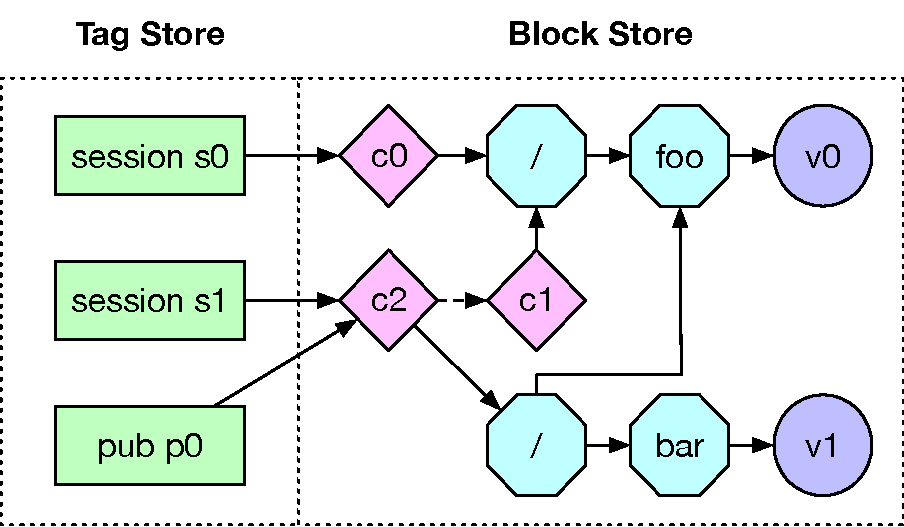
\includegraphics[scale=0.4]{figures/irmin_store}
	\caption{A sample Irmin store. The rectangles are tags, diamonds are commit
	objects, octagons are tree object, and circles are blob objects.}
	\vspace{-0.8cm}
	\label{fig:irmin_store}
\end{wrapfigure}
The expressivity of Irmin imposes significant burden on the underlying storage.
For efficiently storing different versions of the state as the store evolves,
Irmin uses the Git object model. Figure~\ref{fig:irmin_store} shows a snapshot
of the state of the Irmin store. There are two kinds of stores: a mutable tag
store and an immutable, content-addressed block store. The tag store records
the branches and the commit that corresponds to this branch. In this example,
we have three branches, |session s0|, |session s1| and |pub p0|.

The block store is content-addressed and has three different kinds of objects:
commits, tree and blobs. A commit object represents a commit, and it may have
several parent commits and a single reference to a tree node. For example, the
commit |c2|'s parent is |c1|, and |c0| and |c1| do not have any parent commits.
The tree object corresponds to directory entries in a filesystem, and
recursively refer to other tree objects or a blob object. Unlike Git, Irmin
allows blob objects to be arbitrary values, not just files. The blob objects
may refer to other blob objects. In the session |s1|, reading the keys
|["foo"]| and |["bar"]| would yield |Some v0| and |Some v1|, respectively.

Observe that all the commits share the tree object |foo| and its descendents,
thanks to the block store being content addressed. Content addressibility of
the block store means that as the store evolves, the contents of the store are
shared between multiple commits, if possible. On the other hand, updating a
value in a deep hierarchy of tree objects would necessitate allocating a new
spine in order to maintain both the old and the new versions. Thus, each write
in \name will turn into several writes to the underlying storage.

\subsection{Cassandra instantiation}

For instantiating \name on Cassandra, we use two tables, one for the tag store
and another for the block store. For the tag store, the key is a |string| (tag)
and the value is a |blob| (hash of the commit node). For the block store, the
key is a |blob| (hash of the content), and the value is a |blob| (content).
Irmin handles the logic necessary to serialize and deserialize the various Git
objects into binary |blob|s and back.

Cassandra replicates the writes to the tag and block tables asynchronously
amongst the replicas. Each replica periodically merges the public branches of
other replicas into its public branch to fetch remote updates. Due to eventual
consistency of Cassandra, it may be the case that not all the objects from a
remote replica are available locally. For example, the merge function may find
a new commit from a remote replica, but the tree object referenced by a commit
object may not available locally. In this situation, \name simply skips merging
this branch in this round. Cassandra ensures that eventually the remote tree
object will arrive at this replica and will be merged in a subsequent remote
refresh operation. Thus, fetching remote updates is a non-blocking operation.

In Irmin, the tag store is update with a compare-and-swap to ensure that
concurrent updates to the same tag should be disallowed. Naively implementing
this in Cassandra would necessitate the use of lightweight transactions and
suffer prohibitive costs. By restricting the \name programming model
(Section~\ref{sec:model}) such that entries in the tag store (in particular,
the tag corresponding to the public branch of the replica) is only updated on
that replica, we remove the necessity for lightweight transactions. Thus, we
do not depend on any special features of Cassandra to realise the \name model,
and \name can be instantiated on any eventually consistent key-value store.

\subsection{Recursive merges}
\label{sec:rec_merge}

A particular challenge in making \name scalable is the problem of recursive
merges. Consider a simple mergeable counter MRDT, whose implementation is:
\begin{lstlisting}
let merge lca v1 v2 =
let old = match lca with None -> 0 | Some v -> v in
v1 + v2 - old
\end{lstlisting}

\begin{wrapfigure}{r}{0.45\textwidth}
	\centering
	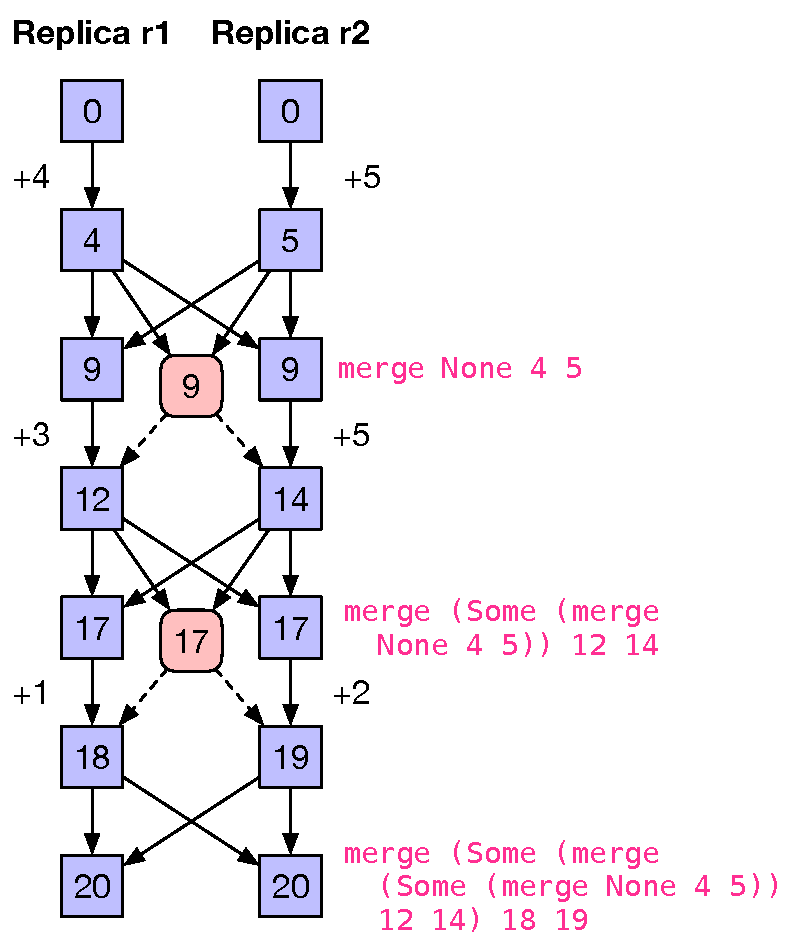
\includegraphics[scale=0.45]{figures/recursive}
	\caption{Recursive merge. Rounded rectangles are the results of recursive
		merges.}
	\label{fig:recursive}
	\vspace{-0.9cm}
\end{wrapfigure}
Consider the execution history presented in Figure~\ref{fig:recursive} which
shows the evolution of a single counter. The history only shows the interaction
between two replicas, and does not show any sessions. Each node in the history
is a commit. Since we want to focus on a single counter, for simplicity, we
ignore the tree nodes and the node labels show the counter value.

Initially the counters are |0|, and each replica concurrently increments the
counter by |4| and |5|. When the replicas perform remote refreshes, they invoke
|merge None 4 5| to resolve the conflict updates yielding |9|. The LCA is
|None| since there is no common ancestor.

Subsequently, the replicas increment the counters by |3| and |5|. Now, consider
that the replicas merge each other's branches. When merging |12| and |14|,
there are two equally valid LCAs |4| and |5|. Picking either one of them leads
to incorrect result. At this point, Irmin merges the two LCAs             using
|merge None 4 5| to yield |9|, which is used as the LCA for merging |12| and
|14|. This yields the value |17|. The result of merging the LCAs is represented
as a rounded rectangle. Importantly, the result of the recursive merge |9| is
not a parent commit of |12| and |14| (distinguished by the use of dotted
arrows). This is because the commit nodes are stored in the content-addressed
store, and adding a new parent to the commit node would create a distinct node,
whose hash is different from the original node. Any other nodes that referenced
the original commit node will continue to reference the old node. As a result,
the recursive merges will need to be performed again for subsequent requests!

Consider that the replicas further evolve by incrementing |1| and |2|, yielding
|18| and |19|. When these commits are merged on remote refresh, there are two
LCAs |12| and |14|, which need to be merged. This in turn has two LCAs |4| and
|5|, which need to be merged. Thus, every subsequent recursive merge, which is
very likely since the replicas merge each other's branches, requires repeating
all the previous recursive merges. This does not scale.

We solve this problem by having a separate table in Cassandra that acts as a
cache, recording the result of LCA merges. Whenever \name encounters a
recursive merge, the cache is first consulted before performing the merge. In
this example, when |18| and |19| are being merged, \name first checks whether
the two LCAs |12| and |14| are in the cache. They would not be. This triggers a
recursive merge of LCAs |4| and |5|, whose result is in the cache, and is
reused. The cache is also updated with an entry that records that the merge of
the LCAs |12| and |14| is the commit corresponding to |17|.

\subsection{Garbage collection}
\label{sec:gc}

While traditional database systems only store the most recent version of the
data, \name necessitates that previous versions of the data must also be kept
around for three-way merges. While persistence of prior
versions~\cite{Driscoll86,farinier15} is a useful property for audit and tamper
evidence, the \name API presented here does not provide a way to access earlier
versions. The question then is: when can those prior versions be garbage
collected?

We have not yet implemented the garbage collector for \name on Cassandra, but we
sketch the design here. Git is equipped with a garbage collector (GC) that
considers that any object in the block store that is reachable from the tag
store is alive. Unreachable objects are be deleted. Our aim is to assist the
Git-like GC by pruning the history graph of nodes which will no longer be used.
The key idea is that if a commit node will not be used for LCA computation,
then that commit node may be deleted. Deleting commit nodes will leave dangling
references from its referees, but Irmin can be extended to ignore
dangling references to commit nodes.

\begin{wrapfigure}{r}{0.5\textwidth}
	\vspace{-1cm}
	\centering
	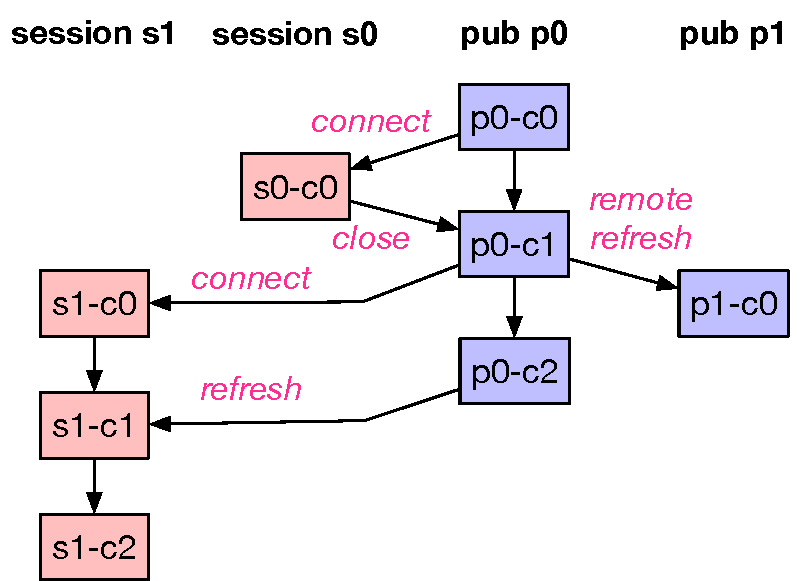
\includegraphics[scale=0.45]{figures/gc}
	\caption{Garbage collection. Here, the commits \texttt{p0-c0} and
		\texttt{s0-c0} may be deleted.}
	\label{fig:gc}
	\vspace{-0.7cm}
\end{wrapfigure}
For individual sessions, once the session is closed, the corresponding entry in
the tag store, and all the commits by that session may be deleted. In the
execution history in Figure~\ref{fig:gc}, the commit node |s0-c0| may be
deleted. The next question is when can commits on public branch be deleted. For
each ongoing session in a replica, we maintain the latest commit in the public
branch against which |refresh| was performed. The earliest of such commits in
the public branch and its descendants must be retained, since they are
necessary for the three-way merge. For example, in Figure~\ref{fig:gc}, session
|s1| refreshed against |p0-c2|, and |s1| is the only ongoing session. If |s1|
publishes, then |p0-c2| will be the LCA commit.

A similar reasoning is used for remote refreshes. When a commit in the public
branch of a replica has been merged into the public branches of all the other
replicas, then the ancestors of such commits will not be accessed and can be
deleted. In Figure~\ref{fig:gc}, assume that we only have two replicas. Since
|p0-c1| was merged by the public branch |p1|, |p0-c1| will be the LCA commit
for subsequent remote refreshes by |p1|. Given that |p0-c0| is neither
necessary for remote refreshes nor for ongoing sessions, |p0-c0| can be
deleted.

%In this section, we evaluate the performance of \name instantiation on
Cassandra. Our goal is to assess the suitability of \name for programming
loosely connected distributed applications. To this end, we first quantify the
overheads of implementing \name over Cassandra. Subsequently, we assess the
performance of MRDTs implemented using \name. And finally, we study the
performance of distributed build cache (Section~\ref{sec:motivation}).

\subsection{Experimental setup}

For the experiments, we use a Cassandra cluster with 4 nodes within the same
data center. Each Cassandra node runs on a baremetal Intel\textregistered
Xeon\textregistered E3-1240 CPU, with 4 physical cores, and 2 hardware threads
per core. Each core runs at 3.70GHz and has 128KB of L1 data cache, 128KB of L1
instruction cache, 1MB L2 cache and 8MB of L3 cache. Each machine has 32GB of
main memory. The machines are unloaded except for the Cassandra node. The ping
latency between the machines is 0.5ms on average. The clients are run on a
machine with the same configuration in the same data center.

For the experiments, Cassandra cluster is configured with a replication factor
of 1, read and write consistency levels of |ONE|. Hence, the cluster maintains
a single copy of each data item, and only waits for one of the servers to
respond to return the result of read and write to the client. These choices
lead to eventual consistency where the reads may not return the latest write.
The cluster may be configured with larger replication factor for better fault
tolerance. However, stronger consistency levels are not useful since \name
enforces per-key causal consistency over the underlying eventual consistency
offered by Cassandra. In fact, choosing strong consistency for reads and writes
in Cassandra does not offer strong consistency in \name since the visibility of
updates in \name is explicitly controlled with the use of |refresh| and
|publish|.

\subsection{Baseline overheads}

\begin{wrapfigure}{r}{0.55\textwidth}
	\vspace{-1cm}
	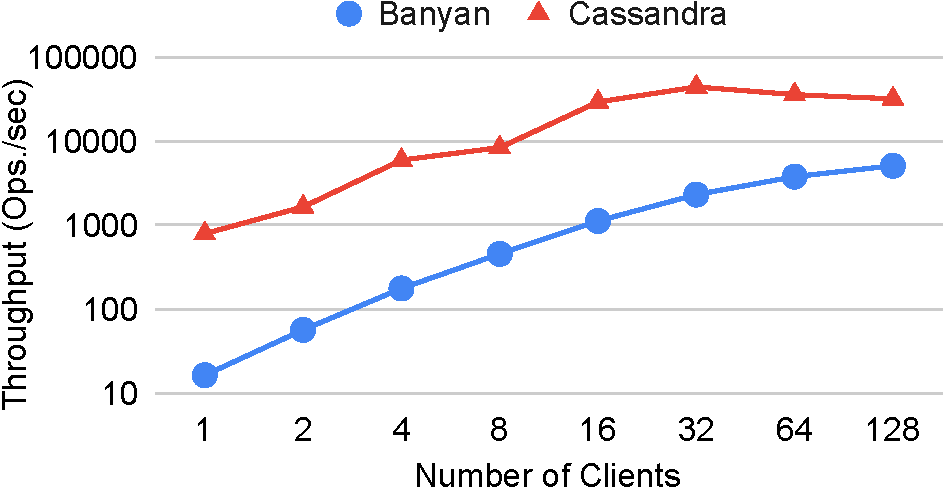
\includegraphics[scale=0.40]{results/baseline}
	\caption{Performance comparison between \name and Cassandra on LWW string
	value.}
	\label{res:baseline}
	\vspace{-0.5cm}
\end{wrapfigure}
Given that \name has to persist every version of the store, what is the impact
of \name when compared to using Cassandra in a scenario where Cassandra would
be sufficient? We measure the throughput of performing 32k operations, with
80\% reads and 20\% writes with different numbers of clients. The keys and
values are 8 and 128 byte strings, respectively. For \name, we use
last-writer-wins resolution policy, which is the policy used by Cassandra. The
results are presented in Figure~\ref{res:baseline}.

With 1 client, \name performs 16 operations per second, while Cassandra
performs 795 operations per second. Cassandra offers 50$\times$ more throughput
than \name with 1 client. This is due to the fact that every read (write)
performs 4 reads (3 reads and 4 writes) to the underlying store to create and
access the tag, commit and tree nodes. \name additionally includes marshalling
and hashing overheads for accessing the content-addressed block store.
Cassandra does not include any of these overheads. Luckily, \name overheads are
local to a client, and hence, can be easily parallelized. With 1 client, the
cluster is severely under utilized, and the client overheads dominate. With
increasing number of clients, the cluster is better utilized. At 128 clients,
Cassandra performs 31274 operations per second where as \name performs 5131
operations per second, which is a slowdown of 6.2$\times$. We believe that
these are reasonable overheads given the stronger consistency and isolation
guarantees, and better programming model offered by \name.

At the end of 32k operations, Cassandra uses 4.9MB of disk space, while \name
uses 1.8GB of disk space. As mentioned earlier (\S\ref{sec:gc}), we have yet to implement garbage collection for
\name -- once implemented, we expect this space usage will come down significantly.

\subsection{Mergeable Types}

\paragraph*{\textbf{Counter}} We begin with the counter data type discussed in
Section~\ref{sec:rec_merge}. How does \name counter perform on when
concurrently updated by multiple clients? For the experiment, the value type is
a counter that supports increment, decrement and read operations. The clients
perform 32k increment or decrement operations on a key randomly selected from a
small key space. Each client refreshes and publishes after every 100
operations. By choosing a small key space, we aim to study the scalability of
the system with large number of conflicts.

\begin{wrapfigure}{r}{0.55\textwidth}
	\vspace{-0.5cm}
	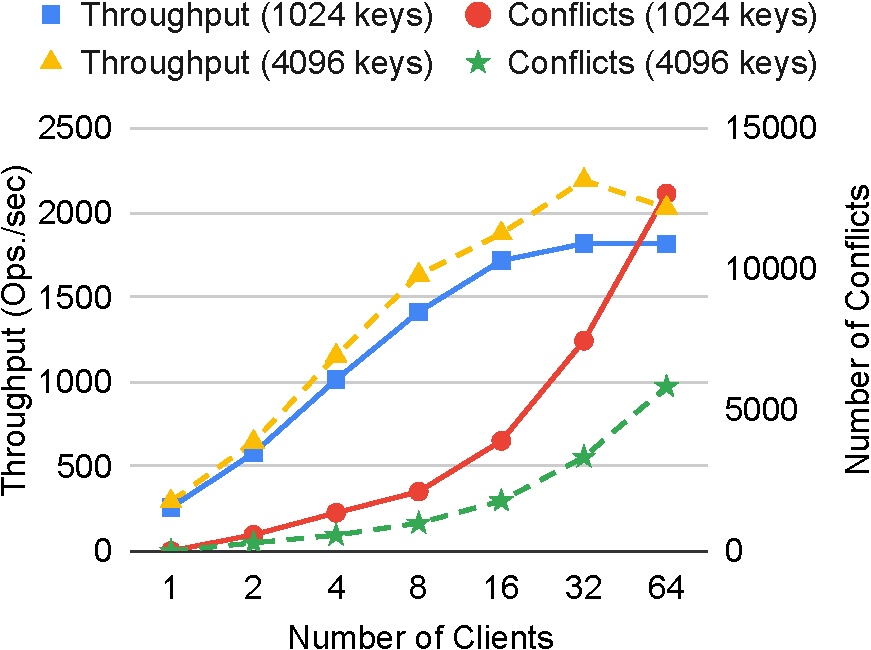
\includegraphics[scale=0.45]{results/counter}
	\caption{Performance of counter MRDT.}
	\label{res:counter}
	\vspace{-0.5cm}
\end{wrapfigure}
Figure~\ref{res:counter} shows the performance result for two key spaces of
size 1024 and 4096 keys. With 1 client, there are no conflicts. The conflicts
increases with increasing number of clients. We get a peak throughput of 1814
(2027) operations per second with a key space of 1024 (4096) keys. Observe that
the number of conflicts is considerably lower with 4096 keys when compared to
1024 keys. As a result, the throughput is higher with 4096 keys. The result
shows that the throughput of the system is proportional to the number of
conflicting operations.

\paragraph*{\textbf{Blob log}} Another useful class of MRDTs are
\emph{mergeable logs}, where each log message is a string. Such a distributed
log is useful for collecting logs in a distributed system, and examining the
logs in their global time order. To this end, each log entry is a pair of
timestamp and message, and the log itself is a list of such entries in reverse
chronological order. The merge function for the mergeable log extracts the
newer log entries from both the versions, sorts the newer entries in reverse
chronological order and returns the list obtained by appending the sorted newer
entries to the front of the log at the LCA.

While this implementation is simple, it does not scale well. In particular,
each commit stores the entire log as a single serialized blob. This does not
take advantage of the fact that every commit can share the tail of the log with
its predecessor. Moreover, every append to the log needs to deserialize the
entire log, append the new entry and serialize the log again. Hence, append is
an $O(n)$ operation, where $n$ is the size of the log. Merges are also worst
case $O(n)$. This is undesirable. We call this implementation a \emph{blob
log}.

\paragraph*{\textbf{Linked log}} We can implement a efficient logs by taking
advantage of the fact that every commit shares the tail of the log with its
predecessor. The value type in this log is:

\begin{lstlisting}
type value =
  | L of float (* timestamp *) * string (* message *)
	     * blob (* hash of prev value *)
	| M of blob list (* hashes of the values being merged *)
\end{lstlisting}

\begin{wrapfigure}{r}{0.4\textwidth}
	\vspace{-1cm}
	\centering
	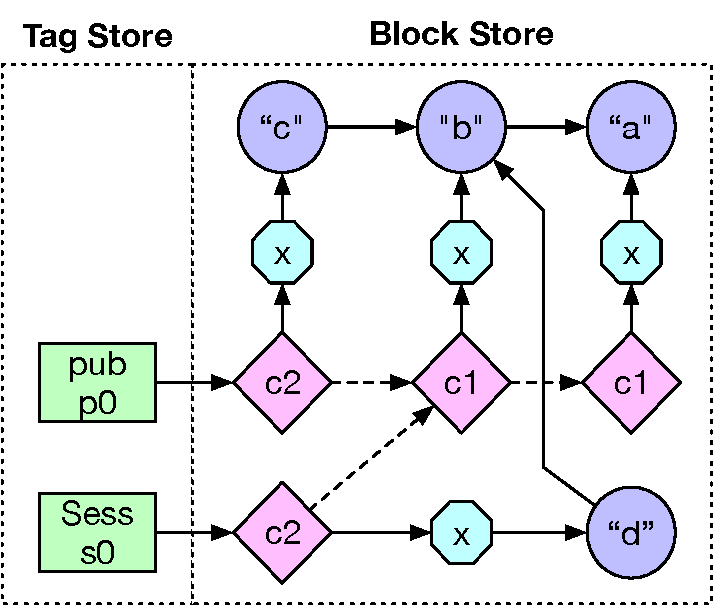
\includegraphics[scale=0.4]{figures/linked_log}
	\caption{A snapshot of linked log storage.}
	\label{fig:linked_log}
	\vspace{-0.5cm}
\end{wrapfigure}
The value is either a log entry |L(t,m,h)| with timestamp |t|, message |m| and
a hash of the previous value |h|. Appending to the log only needs to add a new
object that refers to the previous log value. Hence, append is $O(1)$.
Figure~\ref{fig:linked_log} shows a snapshot of the log assuming a single key
|x|. The log at |x| in the public branch |p0| (session |s0|) is |[a;b;c]|
(|[a;b;d]|). The merge operation simply adds a new value |M [h1;h2]|, which
refers to the hashes of the two log values being merged. This operation is also
$O(1)$. The read function for the log does the heavy-lifting of reading the log
in reverse chronological order.

\begin{wrapfigure}{l}{0.55\textwidth}
	\vspace{-0.5cm}
	\centering
	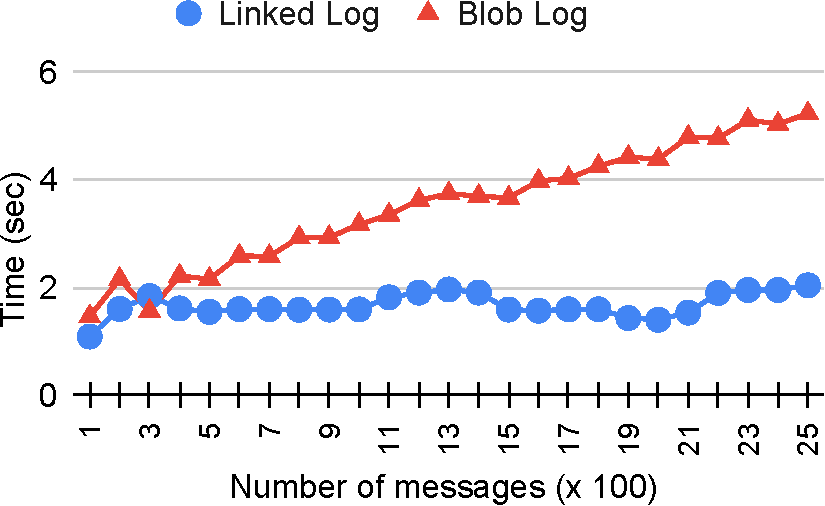
\includegraphics[scale=0.45]{results/log}
	\caption{Performance of mergeable logs.}
	\label{res:log}
	\vspace{-1.5cm}
\end{wrapfigure}
Observe that unlike the examples seen so far where the values do not refer to
other values, this \emph{linked log} implementation refers to other values as
heap data structures would do. Figure~\ref{res:log} shows the time taken to add
100 additional messages to the log with 4 clients. Observe that the time stays
constant with linked log but increases linearly with blob log. By being able to
share objects across different commits (versions), \name leads to efficient
implementations of useful data structures.

\subsection{Distributed build cache}

\begin{wrapfigure}{r}{0.45\textwidth}
	\vspace{-1cm}
	\centering
	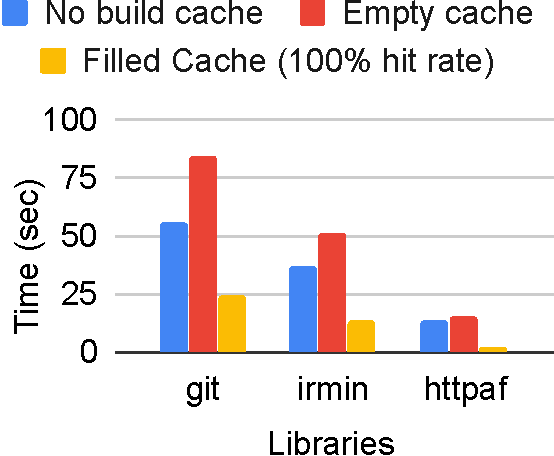
\includegraphics[scale=0.5]{results/build1}
	\caption{Performance of complete reuse of build artefacts.}
	\label{res:build1}
	\vspace{-0.5cm}
\end{wrapfigure}
In this section, we evaluate the performance of distributed build cache
described in Section~\ref{sec:motivation}. We have chosen three OCaml packages:
|git|, |irmin| and |httpaf| with common dependent packages. In the first
experiment, we measure the benefit of building a package that has already been
built in another workspace. Hence, the package artefacts will already be in the
build cache.

For each library, we measure the
baseline build time (1) without using the build cache, (2) using an empty build
cache, and (3) building the same package on a machine with the same package
having built earlier on a different machine. Figure~\ref{res:build1} shows the
results. We see that case using an empty build cache is slower than not using
the cache since the artefacts are stored in the cache. We also see that
building the same package on a different machine is faster due to the build
cache when compared to the baseline.

\begin{wrapfigure}{l}{0.45\textwidth}
	\vspace{-0.5cm}
	\centering
	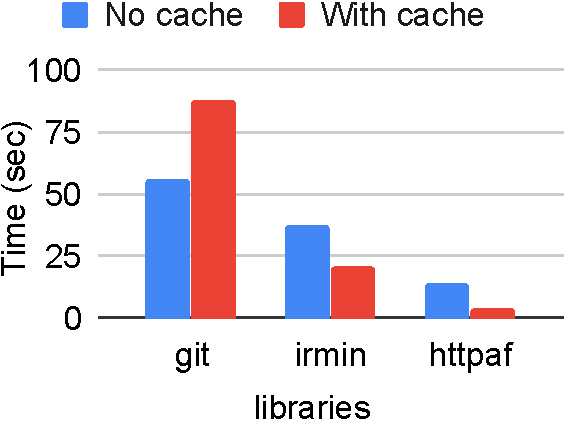
\includegraphics[scale=0.5]{results/build2}
	\caption{Performance of partial reuse of build artefacts.}
	\label{res:build2}
	\vspace{-0.5cm}
\end{wrapfigure}
A more realistic scenario is partial sharing of artefacts, where some of the
dependencies are in the cache and other need to be build locally, and added to
the cache. In this experiment, |git| package is first build on a machine with
an empty cache. Subsequently, |irmin| package is built on a second machine
(which will now benefit from the common artefacts in the cache). And finally,
building |httpaf| on a third machine, which benefits from both of the builds.
Figure~\ref{res:build2} shows the results. As expected, the |git| package build
is slower with cache than without since the cache is empty and the artefacts
need to be written to the cache additionally. Subsequent package builds benefit
from partial sharing of build artefacts. The results illustrate that \name not
only makes it easy to build complex applications like distributed build caches,
but the implementation also performs well under realistic workloads.

%Several prior works have addressed the challenge of balancing the
programmability and performance under eventual consistency. RedBlue
consistency~\cite{Li12} offers causal consistency by default (blue), but
operations that require strong consistency (red) are executed in single total
order. Quelea~\cite{Sivaramakrishnan15} and MixT~\cite{Milano18} offer
automated analysis for classifying and executing operations are different
consistency levels embedded in weakly isolated transactions, paying the cost of
proportional to the consistency level. Indeed, mixing weaker consistency and
transactions have been well-studied~\cite{Brutschy17,Kraska13,CosmosDB}.

\name only supports causal consistency, but it is known to be the strongest
consistency level that remains available~\cite{Llyod11}. While prior works
attempt to reconcile traditional isolation levels with weak consistency, \name
leaves the choice of reading and writing updates to and from other transactions
to the client through the use of |publish| and |refresh|. We believe that
traditional database isolation levels are already quite difficult to get
right~\cite{Kaki17}, and attempting to provide a fixed set of poorly understood
isolation levels under weak consistency will lead to proliferation of bugs.

\name is distinguished by the equipping data types with the ability to handle
conflicts (three-way merge functions). \name builds on top of
Irmin~\cite{Irmin} library. Irmin allows arbitrary branching and merging
between different branches at the cost of having to expose the branch name.
\name refreshes and publishes implicitly to the public branch at a repository,
which obviates the need for naming branches explicitly. Irmin does not include
a distribution and convergence layer; \name uses Cassandra for this purpose.
\name provides causal consistency and coordination free transactions over
weakly consistent Cassandra. Several prior work have similarly obtained
stronger guarantees weaker stores~\cite{Sivaramakrishnan15,Bailis13b}.

TARDiS~\cite{Crooks16} supports user-defined data types, and a transaction
model similar to \name. TARDiS is however a machine model that exposes the
details of explicit branches and merges to the developer, whereas \name is a
programming model that can be instantiated on any eventually consistent
key-value store. For instance, in TARDiS programmers need to invoke a separate
merge transaction that does an n-way merge. \name transaction model is more
flexible than TARDiS. For example, \name can support monotonic atomic view,
which TARDiS cannot -- TARDiS transactions do not have a way of allowing more
recent updates since the transaction began. TARDiS does not discuss merges
without LCAs or the issue with recursive merges. We found recursive merges to
be a very common occurrence in practice. Concurrent
revisions~\cite{Burckhardt12} describe a programming model with branch and
merge workflow with explicit branches and restrictions on the shape of history
graphs. \name makes the choice of branches to publish and refresh implicit
leading to a simpler model. Concurrent revisions does not include an
implementation.

%\section{Conclusion}
\label{sec:conc}

We present \name, a novel programming model for developing loosely connected
distributed applications based on the principles of Git. We illustrate the
practicality of this approach by instantiating \name on Cassandra, an
off-the-shelf eventually consistent distributed store. Our experimental results
suggests that \name makes it easy to build complex distributed applications
without compromising performance.
%\input{simulation-exp.tex}
%\input{cvar-results.tex}
%\input{conclusions.tex}
%\input{appendix.tex}
%%%%%%%%%%%%%%%%%%%%%%%%%%%%%%%%%%%%%%%%%%%%%%%%%%%
% Introduction.
\chapter{Zero}
\label{chap:zero}

This document provides a simple template of how the provided
\verb+iitmdiss.cls+ \LaTeX\ class is to be used.  Also provided are
several useful tips to do various things that might be of use when you
write your thesis.

Before reading any further please note that you are strongly advised
against changing any of the formatting options used in the class
provided in this directory, unless you are absolutely sure that it
does not violate the IITM formatting guidelines.  \emph{Please do not
  change the margins or the spacing.}  If you do change the formatting
you are on your own (don't blame me if you need to reprint your entire
thesis).  In the case that you do change the formatting despite these
warnings, the least I ask is that you do not redistribute your style
files to your friends (or enemies).

It is also a good idea to take a quick look at the formatting
guidelines.  Your office or advisor should have a copy.  If they
don't, pester them, they really should have the formatting guidelines
readily available somewhere.

To compile your sources run the following from the command line:
\begin{verbatim}
% latex thesis.tex
% bibtex thesis
% latex thesis.tex
% latex thesis.tex
\end{verbatim}
Modify this suitably for your sources.

To generate PDF's with the links from the \verb+hyperref+ package use
the following command:
\begin{verbatim}
% dvipdfm -o thesis.pdf thesis.dvi
\end{verbatim}

\section{Package Options}

Use this thesis as a basic template to format your thesis.  The
\verb+iitmdiss+ class can be used by simply using something like this:
\begin{verbatim}
\documentclass[PhD]{iitmdiss}  
\end{verbatim}

To change the title page for different degrees just change the option
from \verb+PhD+ to one of \verb+MS+, \verb+MTech+ or \verb+BTech+.
The dual degree pages are not supported yet but should be quite easy
to add.  The title page formatting really depends on how large or
small your thesis title is.  Consequently it might require some hand
tuning.  Edit your version of \verb+iitmdiss.cls+ suitably to do this.
I recommend that this be done once your title is final.

To write a synopsis simply use the \verb+synopsis.tex+ file as a
simple template.  The synopsis option turns this on and can be used as
shown below.
\begin{verbatim}
\documentclass[PhD,synopsis]{iitmdiss}                                
\end{verbatim}

Once again the title page may require some small amount of fine
tuning.  This is again easily done by editing the class file.

This sample file uses the \verb+hyperref+ package that makes all
labels and references clickable in both the generated DVI and PDF
files.  These are very useful when reading the document online and do
not affect the output when the files are printed.


\section{Example Figures and tables}

Fig.~\ref{fig:iitm} shows a simple figure for illustration along with
a long caption.  The formatting of the caption text is automatically
single spaced and indented.  Table~\ref{tab:sample} shows a sample
table with the caption placed correctly.  The caption for this should
always be placed before the table as shown in the example.


\begin{figure}[htpb]
  \begin{center}
    \resizebox{50mm}{!} {\includegraphics *{iitm.eps}}
    \resizebox{50mm}{!} {\includegraphics *{iitm.eps}}
    \caption {Two IITM logos in a row.  This is also an
      illustration of a very long figure caption that wraps around two
      two lines.  Notice that the caption is single-spaced.}
  \label{fig:iitm}
  \end{center}
\end{figure}

\begin{table}[htbp]
  \caption{A sample table with a table caption placed
    appropriately. This caption is also very long and is
    single-spaced.  Also notice how the text is aligned.}
  \begin{center}
  \begin{tabular}[c]{|c|r|} \hline
    $x$ & $x^2$ \\ \hline
    1  &  1   \\
    2  &  4  \\
    3  &  9  \\
    4  &  16  \\
    5  &  25  \\
    6  &  36  \\
    7  &  49  \\
    8  &  64  \\ \hline
  \end{tabular}
  \label{tab:sample}
  \end{center}
\end{table}

\section{Bibliography with BIB\TeX}

I strongly recommend that you use BIB\TeX\ to automatically generate
your bibliography.  It makes managing your references much easier.  It
is an excellent way to organize your references and reuse them.  You
can use one set of entries for your references and cite them in your
thesis, papers and reports.  If you haven't used it anytime before
please invest some time learning how to use it.  

I've included a simple example BIB\TeX\ file along in this directory
called \verb+refs.bib+.  The \verb+iitmdiss.cls+ class package which
is used in this thesis and for the synopsis uses the \verb+natbib+
package to format the references along with a customized bibliography
style provided as the \verb+iitm.bst+ file in the directory containing
\verb+thesis.tex+.  Documentation for the \verb+natbib+ package should
be available in your distribution of \LaTeX.  Basically, to cite the
author along with the author name and year use \verb+\cite{key}+ where
\verb+key+ is the citation key for your bibliography entry.  You can
also use \verb+\citet{key}+ to get the same effect.  To make the
citation without the author name in the main text but inside the
parenthesis use \verb+\citep{key}+.  The following paragraph shows how
citations can be used in text effectively.

More information on BIB\TeX\ is available in the book by
\cite{lamport:86}.  There are many
references~\citep{lamport:86,prabhu:xx} that explain how to use
BIB\TeX.  Read the \verb+natbib+ package documentation for more
details on how to cite things differently.

Here are other references for example.  \citet{viz:mayavi} presents a
Python based visualization system called MayaVi in a conference paper.
\citet{pan:pr:flat-fst} illustrates a journal article with multiple
authors.  Python~\citep{py:python} is a programming language and is
cited here to show how to cite something that is best identified with
a URL.

\section{Other useful \LaTeX\ packages}

The following packages might be useful when writing your thesis.

\begin{itemize}  
\item It is very useful to include line numbers in your document.
  That way, it is very easy for people to suggest corrections to your
  text.  I recommend the use of the \texttt{lineno} package for this
  purpose.  This is not a standard package but can be obtained on the
  internet.  The directory containing this file should contain a
  lineno directory that includes the package along with documentation
  for it.

\item The \texttt{listings} package should be available with your
  distribution of \LaTeX.  This package is very useful when one needs
  to list source code or pseudo-code.

\item For special figure captions the \texttt{ccaption} package may be
  useful.  This is specially useful if one has a figure that spans
  more than two pages and you need to use the same figure number.

\item The notation page can be entered manually or automatically
  generated using the \texttt{nomencl} package.

\end{itemize}

More details on how to use these specific packages are available along
with the documentation of the respective packages.


%%%%%%%%%%%%%%%%%%%%%%%%%%%%%%%%%%%%%%%%%%%%%%%%%%%%%%%%%%%%
% Appendices.

\appendix

\chapter{A SAMPLE APPENDIX}

Just put in text as you would into any chapter with sections and
whatnot.  Thats the end of it.

%%%%%%%%%%%
%%%%%%%%%%%
%%%%%%%%%%%


%%%%%%%%%%%%%%%%%%%%%%%%%%%%%%%%%%%%%%%%%%%%%%%%%%%%%%%%%%%%
% Bibliography.

\begin{singlespace}
  \bibliography{banyan}
\end{singlespace}


%%%%%%%%%%%%%%%%%%%%%%%%%%%%%%%%%%%%%%%%%%%%%%%%%%%%%%%%%%%%
% List of papers

\listofpapers

%\begin{enumerate}  
%\item A. K. Pandey, L. A. Prashanth and S. P. Bhat,  \newblock
%\textit{Estimation of Spectral Risk Measures}, under review in Operation research letters, and preprint is available on arXiv:1912.10398
  %\newblock {\em Journal}, Volume,
  %Page, (year).
%\end{enumerate}  

\end{document}
